% =============================================================
%  Chapter — AC power transmission
%  This file holds the chapter heading and its introduction only; the
%  content is one file per subsection, \input below in reading order:
%    fundamentals.tex         the general two-port representation
%    overhead-lines.tex       what sets R', L', G', C' on an OHL
%    cables.tex               what changes against an overhead line
%    reference-line.tex       the 500 kV worked example
%    natural-power.tex        surge-impedance loading
%    transmission-limits.tex  thermal, voltage drop, stability
%    angular-stability.tex    synchronising power and the margin
%    series-compensation.tex  shortening the electrical length
%  Figures of this chapter are in fig/ next to this file; their
%  generating scripts are named in the sub-file header comments.
%  Matching slides: presentation/design/ac-transmission/
% =============================================================
\section{AC Power Transmission}
\label{sec:ac-chapter}

The familiar statement that active power flows on the angle between two
voltages, $P = U_S \cdot U_R / X \cdot \sin\delta$, is a special case. It
holds for a short, lossless line, and its error grows with length.

This chapter builds the representation from the line parameters upwards and
then applies it. Section~\ref{sec:ac-transmission} gives the general form:
the four per-unit-length quantities, the two-port that follows from them,
the exact power transfer relation, the conditions under which it collapses
to the simple form, and the distributed solution that replaces the lumped
one on long lines. Sections~\ref{sec:ohl} and~\ref{sec:cable} give the
parameters of an overhead line and of a cable, and
Section~\ref{sec:reference-line} carries the chain through on one worked
example. Sections~\ref{sec:natural-power} to~\ref{sec:series-compensation}
apply the representation: the natural power, the three transmission limits,
the angular stability margin and the effect of series compensation.

% =============================================================
%  AC power transmission — the general representation
%  Applies to overhead lines and cables alike; the type-specific
%  parameters are in overhead-lines.tex and cables.tex, the worked
%  numbers in reference-line.tex.
%  Figures: the nominal pi-section in the per-unit-length parameters,
%  the same section as a two-port, and the terminal quantities with
%  the coordinate x -- all inline TikZ in the report colours.
% =============================================================
\subsection{Fundamentals}
\label{sec:ac-transmission}

Nothing in this section distinguishes an overhead line from a cable. The two
differ only in the values of the four parameters and in what those values
make critical; Section~\ref{sec:ohl} covers the overhead line and
Section~\ref{sec:cable} the cable.


\subsubsection{Line parameters}
\label{sec:ac-parameters}

A transmission line is described by four parameters per unit length, two in
series with the conductor and two in shunt to the return path. Each
corresponds to one physical effect, Table~\ref{tab:ac-parameters}.

\begin{table}[!ht]
  \centering
  \begin{tabularx}{\linewidth}{@{}l l X@{}}
    \toprule
    & \multicolumn{1}{c}{\textbf{Parameter}} & \textbf{Physical effect} \\
    \midrule
    $R'$ & Resistance  & Ohmic loss in the conductors \\
    $L'$ & Inductance  & Magnetic field around the conductors \\
    $G'$ & Conductance & Leakage through the insulation and corona \\
    $C'$ & Capacitance & Electric field to the other conductors and to earth \\
    \bottomrule
  \end{tabularx}
  \caption{Line parameters per unit length}
  \label{tab:ac-parameters}
\end{table}

They enter as a series impedance and a shunt admittance per unit length,
\begin{equation}
  \underline{Z}' = R' + j \cdot \omega \cdot L'
  \qquad
  \underline{Y}' = G' + j \cdot \omega \cdot C'
  \label{eq:ac-zy-prime}
\end{equation}

$R'$ and $L'$ follow from the conductor itself and from the arrangement of
the conductors; $G'$ and $C'$ from the insulation between them. The
expressions differ between an overhead line and a cable and are given in
Sections~\ref{sec:ohl} and~\ref{sec:cable}.

Taken over a finite length the four parameters arrange themselves as the
nominal $\pi$-section of Figure~\ref{fig:ac-pi-section}: the series branch
carries $R'$ and $L'$, and the shunt branch $G'$ and $C'$ is split equally
between the two ends.

\begin{figure}[!ht]
  \centering
  \begin{tikzpicture}[
      x=0.60cm, y=0.60cm, line width=0.8pt,
      every node/.style={inner sep=1.5pt, font=\small},
      rail/.style={atFg, line width=0.8pt},
      box/.style={draw=atFg, fill=atBgSubtle, line width=0.8pt,
                  minimum width=1.0cm, minimum height=0.46cm},
      vbox/.style={draw=atFg, fill=atBgSubtle, line width=0.8pt,
                   minimum width=0.60cm, minimum height=1.05cm},
      term/.style={circle, draw=atFg, fill=white, line width=0.8pt,
                   minimum size=3.8pt, inner sep=0pt},
      dim/.style={dotted, atFgMuted, line width=0.9pt},
      ext/.style={<->, >=Latex, atFgMuted, line width=0.8pt},
    ]
    % series branch
    \draw[rail] (0,2.8) -- (2.77,2.8);
    \node[box] at (3.6,2.8) {$R'$};
    \draw[rail] (4.43,2.8) -- (4.77,2.8);
    \node[box] at (5.6,2.8) {$L'$};
    \draw[rail] (6.43,2.8) -- (9.2,2.8);
    % return conductor
    \draw[rail] (0,0) -- (9.2,0);
    % left shunt leg
    \draw[rail] (1.3,2.8) -- (1.3,2.4);
    \draw[rail] (0.7,2.4) -- (1.9,2.4);
    \draw[rail] (0.7,2.4) -- (0.7,2.28);
    \draw[rail] (1.9,2.4) -- (1.9,2.28);
    \node[vbox] at (0.7,1.4) {$\frac{G'}{2}$};
    \node[vbox] at (1.9,1.4) {$\frac{C'}{2}$};
    \draw[rail] (0.7,0.52) -- (0.7,0.4);
    \draw[rail] (1.9,0.52) -- (1.9,0.4);
    \draw[rail] (0.7,0.4) -- (1.9,0.4);
    \draw[rail] (1.3,0.4) -- (1.3,0);
    % right shunt leg
    \draw[rail] (7.9,2.8) -- (7.9,2.4);
    \draw[rail] (7.3,2.4) -- (8.5,2.4);
    \draw[rail] (7.3,2.4) -- (7.3,2.28);
    \draw[rail] (8.5,2.4) -- (8.5,2.28);
    \node[vbox] at (7.3,1.4) {$\frac{G'}{2}$};
    \node[vbox] at (8.5,1.4) {$\frac{C'}{2}$};
    \draw[rail] (7.3,0.52) -- (7.3,0.4);
    \draw[rail] (8.5,0.52) -- (8.5,0.4);
    \draw[rail] (7.3,0.4) -- (8.5,0.4);
    \draw[rail] (7.9,0.4) -- (7.9,0);
    % terminals
    \node[term] at (0,2.8) {};    \node[term] at (0,0) {};
    \node[term] at (9.2,2.8) {};  \node[term] at (9.2,0) {};
    % length
    \draw[dim] (0,-0.3) -- (0,-1.6);
    \draw[dim] (9.2,-0.3) -- (9.2,-1.6);
    \draw[ext] (0,-1.2) -- (9.2,-1.2);
    \node[below=1pt, atFgMuted] at (4.6,-1.2) {$l$};
  \end{tikzpicture}
  \caption{Nominal $\pi$-section of a line of length $l$, written in the
           per-unit-length parameters}
  \label{fig:ac-pi-section}
\end{figure}

\subsubsection{The line as a two-port}
\label{sec:ac-two-port}

Over a length $l$ the parameters give a series impedance and a shunt
admittance
\begin{equation}
  \underline{Z} = \underline{Z}' \cdot l
  \qquad
  \underline{Y} = \underline{Y}' \cdot l
  \label{eq:ac-zy}
\end{equation}

\begin{figure}[!ht]
  \centering
  \begin{tikzpicture}[
      x=0.75cm, y=0.75cm, line width=0.8pt,
      every node/.style={inner sep=1.5pt, font=\small},
      rail/.style={atFg, line width=0.8pt},
      box/.style={draw=atFg, fill=atBgSubtle, line width=0.8pt,
                  minimum width=1.1cm, minimum height=0.46cm},
      vbox/.style={draw=atFg, fill=atBgSubtle, line width=0.8pt,
                   minimum width=0.55cm, minimum height=1.1cm},
      term/.style={circle, draw=atFg, fill=white, line width=0.8pt,
                   minimum size=3.8pt, inner sep=0pt},
      flow/.style={->, >=Latex, atFg, line width=0.8pt},
    ]
    % series branch
    \draw[rail] (0,2.6) -- (2.27,2.6);
    \node[box] at (3,2.6) {$\underline{Z}$};
    \draw[rail] (3.73,2.6) -- (6,2.6);
    % return conductor
    \draw[rail] (0,0) -- (6,0);
    % shunt legs
    \draw[rail] (1.2,2.6) -- (1.2,2.035);
    \node[vbox] at (1.2,1.3) {$\frac{\underline{Y}}{2}$};
    \draw[rail] (1.2,0.565) -- (1.2,0);
    \draw[rail] (4.8,2.6) -- (4.8,2.035);
    \node[vbox] at (4.8,1.3) {$\frac{\underline{Y}}{2}$};
    \draw[rail] (4.8,0.565) -- (4.8,0);
    % terminals
    \node[term] at (0,2.6) {};  \node[term] at (0,0) {};
    \node[term] at (6,2.6) {};  \node[term] at (6,0) {};
    % terminal currents
    \draw[flow] (-1.0,2.6) -- (-0.4,2.6);
    \node[left] at (-1.15,2.6) {$\underline{I}_S$};
    \draw[flow] (6.4,2.6) -- (7.0,2.6);
    \node[right] at (7.15,2.6) {$\underline{I}_R$};
    % terminal voltages, inset so they clear the terminals
    \draw[flow] (0,2.25) -- (0,0.35);
    \node[left=2pt] at (0,1.3) {$\underline{U}_S$};
    \draw[flow] (6,2.25) -- (6,0.35);
    \node[right=2pt] at (6,1.3) {$\underline{U}_R$};
  \end{tikzpicture}
  \caption{The same $\pi$-section as a two-port: the whole series impedance
           $\underline{Z}$ between the rails, half the shunt admittance
           $\underline{Y}$ at each end}
  \label{fig:ac-pi-zy}
\end{figure}

which the nominal $\pi$ arranges as in Figure~\ref{fig:ac-pi-zy}: the whole
series impedance between the rails and half the shunt admittance at each
end. This is the standard two-port description of a linear network, of which
the line is one case; Appendix~\ref{sec:two-port} gives the general form for
the reader who wants it, and is not needed here. The ports are named by
function throughout this section, the sending end and the receiving end. The
line is then a two-port,
\begin{equation}
  \begin{bmatrix} \underline{U}_S \\ \underline{I}_S \end{bmatrix}
  =
  \begin{bmatrix} \underline{A} & \underline{B} \\
                  \underline{C} & \underline{D} \end{bmatrix}
  \cdot
  \begin{bmatrix} \underline{U}_R \\ \underline{I}_R \end{bmatrix}
  \label{eq:ac-abcd}
\end{equation}
with, for the nominal $\pi$,
\begin{equation}
  \underline{A} = \underline{D} = 1 + \frac{\underline{Z} \cdot \underline{Y}}{2},
  \qquad
  \underline{B} = \underline{Z},
  \qquad
  \underline{C} = \underline{Y} \cdot
      \left(1 + \frac{\underline{Z} \cdot \underline{Y}}{4}\right)
  \label{eq:ac-abcd-pi}
\end{equation}

The shunt admittance appears in $\underline{A}$. A line with no shunt
capacitance has $\underline{A} = 1$ and behaves as a single series
impedance; the departure of $\left|\underline{A}\right|$ from unity
measures the departure from that case.

\subsubsection{Power transfer}
\label{sec:ac-power-transfer}

Solving~\eqref{eq:ac-abcd} for the receiving-end current gives
\begin{equation}
  \underline{I}_R
    = \frac{\underline{U}_S - \underline{A} \cdot \underline{U}_R}
           {\underline{B}}
  \label{eq:ac-ir}
\end{equation}
Taking the receiving-end voltage as the phase reference, so that $\delta$ is
the angle by which the sending-end voltage leads it,
\begin{equation}
  \underline{U}_S = U_S \cdot e^{\,j \cdot \delta},
  \quad
  \underline{U}_R = U_R,
  \quad
  \underline{A} = \left|A\right| \cdot e^{\,j \cdot \vartheta_A},
  \quad
  \underline{B} = \left|B\right| \cdot e^{\,j \cdot \vartheta_B}
  \label{eq:ac-reference}
\end{equation}
the receiving-end complex power $\underline{S}_R = \underline{U}_R \cdot
\underline{I}_R^{*}$ separates into
\begin{align}
  P_R &= \frac{U_S \cdot U_R}{\left|B\right|}
         \cdot \cos\left(\vartheta_B - \delta\right)
       - \frac{\left|A\right| \cdot U_R^2}{\left|B\right|}
         \cdot \cos\left(\vartheta_B - \vartheta_A\right)
  \label{eq:ac-pr} \\[0.3em]
  Q_R &= \frac{U_S \cdot U_R}{\left|B\right|}
         \cdot \sin\left(\vartheta_B - \delta\right)
       - \frac{\left|A\right| \cdot U_R^2}{\left|B\right|}
         \cdot \sin\left(\vartheta_B - \vartheta_A\right)
  \label{eq:ac-qr}
\end{align}
with $U_S$ and $U_R$ line-to-line magnitudes, so that $P_R$ and $Q_R$ are
three-phase quantities.

Two numbers carry the whole behaviour of the line. The angle $\vartheta_B$
sets where the maximum of $P_R$ falls: differentiating~\eqref{eq:ac-pr} puts
it at $\delta = \vartheta_B$, which is $90^\circ$ only for a lossless line.
The magnitude $\left|A\right|$ scales the second term, a constant offset
independent of $\delta$ that exists only because the line charges itself.

\subsubsection{The short, lossless line}
\label{sec:ac-simplified}

For a short line the shunt admittance vanishes and $\underline{A} =
\underline{D} = 1$, so $\left|A\right| = 1$ and $\vartheta_A = 0$. For a
lossless line $\underline{B} = \underline{Z} = j \cdot X$, so
$\left|B\right| = X$ and $\vartheta_B = 90^\circ$. With
$\cos\left(90^\circ - \delta\right) = \sin\delta$ and $\cos 90^\circ = 0$,
equations~\eqref{eq:ac-pr} and~\eqref{eq:ac-qr} collapse to
\begin{equation}
  P = \frac{U_S \cdot U_R}{X} \cdot \sin\delta
  \qquad
  Q_R = \frac{U_S \cdot U_R \cdot \cos\delta - U_R^2}{X}
  \label{eq:ac-simple}
\end{equation}
with the series reactance
\begin{equation}
  X = \omega \cdot L' \cdot l
  \label{eq:ac-x}
\end{equation}

For small angles this separates further into
$P \approx U_S \cdot U_R \cdot \delta / X$ and
$Q_R \approx U_R \cdot \left(U_S - U_R\right) / X$: active power is carried
by the angle between the terminal voltages, reactive power by the difference
in their magnitude. The decoupling holds for small angles and is the basis
for treating the two separately in estimation, although~\eqref{eq:ac-simple}
is not accurate enough to compute with on a long line.

The $X$ of~\eqref{eq:ac-simple} is not the line alone but the whole path
between the two internal voltages --- the source impedances and the
transformers at both ends are in series with it --- so the short-circuit
level at the terminals belongs in any statement of transfer capability.

\subsubsection{Distributed representation}
\label{sec:ac-wave}

The $\pi$-section lumps parameters that are distributed along the line. The distributed description uses two quantities,
\begin{equation}
  \underline{\gamma} = \alpha + j \cdot \beta
    = \sqrt{\underline{Z}' \cdot \underline{Y}'}
  \qquad
  \underline{Z}_w = \sqrt{\frac{\underline{Z}'}{\underline{Y}'}}
  \label{eq:ac-gamma-zw}
\end{equation}
the propagation constant and the wave impedance. Voltage and current are
then defined at every cross-section of the line rather than only at its
terminals, Figure~\ref{fig:ac-terminals}. At a distance $x$ from the
sending end of a line of length $l$ they are
\begin{align}
  \underline{U} &= \underline{U}_R \cdot
      \cosh\left(\underline{\gamma} \cdot \left(l-x\right)\right)
    + \underline{Z}_w \cdot \underline{I}_R \cdot
      \sinh\left(\underline{\gamma} \cdot \left(l-x\right)\right)
  \label{eq:ac-u-x} \\[0.3em]
  \underline{I} &= \frac{\underline{U}_R}{\underline{Z}_w} \cdot
      \sinh\left(\underline{\gamma} \cdot \left(l-x\right)\right)
    + \underline{I}_R \cdot
      \cosh\left(\underline{\gamma} \cdot \left(l-x\right)\right)
  \label{eq:ac-i-x}
\end{align}

\begin{figure}[!ht]
  \centering
  \begin{tikzpicture}[
      x=0.62cm, y=0.62cm, line width=0.8pt,
      every node/.style={inner sep=1.5pt, font=\small},
      rail/.style={atFg, line width=0.8pt},
      term/.style={circle, draw=atFg, fill=atBg, line width=0.8pt,
                   minimum size=4.5pt, inner sep=0pt},
      flow/.style={atFg, -{Triangle[length=2.4mm,width=2.0mm]},
                   line width=0.8pt},
      dim/.style={atFgMuted, dotted, line width=0.9pt},
      ext/.style={atFgMuted, {Stealth[length=1.6mm]}-{Stealth[length=1.6mm]},
                  line width=0.6pt},
    ]
    \def\xa{0}\def\xb{9}\def\xm{3.3}\def\yt{3.6}\def\yb{0}
    % conductors
    \draw[rail] (\xa,\yt) -- (\xb,\yt);
    \draw[rail] (\xa,\yb) -- (\xb,\yb);
    % line current at the cross-section
    \draw[flow] (\xa,\yt) -- (\xm,\yt);
    \node[above=1pt] at (\xm,\yt) {$\underline{I}$};
    % terminals
    \node[term] at (\xa,\yt) {};  \node[term] at (\xb,\yt) {};
    \node[term] at (\xa,\yb) {};  \node[term] at (\xb,\yb) {};
    % terminal currents
    \draw[flow] ({\xa-1.7},\yt) -- ({\xa-0.8},\yt);
    \node[left] at ({\xa-1.9},\yt) {$\underline{I}_S$};
    \draw[flow] ({\xb+0.8},\yt) -- ({\xb+1.7},\yt);
    \node[right] at ({\xb+1.9},\yt) {$\underline{I}_R$};
    % voltages, upper conductor to lower conductor
    \draw[flow] (\xa,{\yt-0.4}) -- (\xa,{\yb+0.4});
    \node[right=2pt] at (\xa,{(\yt+\yb)/2}) {$\underline{U}_S$};
    \draw[flow] (\xm,{\yt-0.4}) -- (\xm,{\yb+0.4});
    \node[right=2pt] at (\xm,{(\yt+\yb)/2}) {$\underline{U}$};
    \draw[flow] (\xb,{\yt-0.4}) -- (\xb,{\yb+0.4});
    \node[right=2pt] at (\xb,{(\yt+\yb)/2}) {$\underline{U}_R$};
    % coordinate x and total length l
    \draw[dim] (\xa,{\yb-0.3}) -- (\xa,{\yb-2.6});
    \draw[dim] (\xm,{\yb-0.3}) -- (\xm,{\yb-1.6});
    \draw[dim] (\xb,{\yb-0.3}) -- (\xb,{\yb-2.6});
    \draw[ext] (\xa,{\yb-1.2}) -- (\xm,{\yb-1.2});
    \node[below=1pt, atFgMuted] at ({(\xa+\xm)/2},{\yb-1.2}) {$x$};
    \draw[ext] (\xa,{\yb-2.2}) -- (\xb,{\yb-2.2});
    \node[below=1pt, atFgMuted] at ({(\xa+\xb)/2},{\yb-2.2}) {$l$};
  \end{tikzpicture}
  \caption{Terminal quantities of the two-port and the local voltage and
           current at a distance $x$ along the line}
  \label{fig:ac-terminals}
\end{figure}

Evaluating~\eqref{eq:ac-u-x} and~\eqref{eq:ac-i-x} at $x = 0$ and comparing
with~\eqref{eq:ac-abcd} identifies the exact two-port parameters,
\begin{equation}
  \underline{A} = \underline{D} = \cosh\left(\underline{\gamma} \cdot l\right),
  \qquad
  \underline{B} = \underline{Z}_w \cdot
      \sinh\left(\underline{\gamma} \cdot l\right),
  \qquad
  \underline{C} = \frac{\sinh\left(\underline{\gamma} \cdot l\right)}
                       {\underline{Z}_w}
  \label{eq:ac-abcd-exact}
\end{equation}
which replace the nominal-$\pi$ entries of~\eqref{eq:ac-abcd-pi}. The
relations~\eqref{eq:ac-pr} and~\eqref{eq:ac-qr} are unchanged; only the way
$\underline{A}$ and $\underline{B}$ are computed differs.

The exact result can itself be written as a $\pi$. Matching the branches of a
$\pi$-section to~\eqref{eq:ac-abcd-exact} entry by entry gives
\begin{equation}
  \underline{Z}_{eq} = \underline{Z}_w \cdot
      \sinh\left(\underline{\gamma} \cdot l\right),
  \qquad
  \frac{\underline{Y}_{eq}}{2} = \frac{1}{\underline{Z}_w} \cdot
      \tanh\left(\frac{\underline{\gamma} \cdot l}{2}\right)
  \label{eq:ac-equivalent-pi}
\end{equation}
the \emph{equivalent} $\pi$, often called the long-line correction. It is not
an approximation: one $\pi$ with these two branches reproduces the
distributed line exactly at its terminals at that frequency, because
$1 + \sinh\left(\underline{\gamma} \cdot l\right) \cdot
\tanh\left(\underline{\gamma} \cdot l / 2\right) =
\cosh\left(\underline{\gamma} \cdot l\right)$. The nominal $\pi$
of~\eqref{eq:ac-abcd-pi} is its small-argument limit, with
$\sinh u \to u$ and $\tanh u \to u$. This is what a load-flow program
stores for a long line, and it allows a $\pi$-shaped model at any
length. Section~\ref{sec:ref-cascade} puts numbers on both.

What decides whether the lumped form will do is the electrical length
$\beta \cdot l$, not the length in km. Since $\beta = \omega \cdot
\sqrt{L' \cdot C'}$ for a low-loss line, a cable reaches a given electrical
length in a fraction of the distance an overhead line needs, and the lumped
approximation fails correspondingly earlier.

\FloatBarrier

% =============================================================
%  Overhead lines — what sets R', L', G', C' on an OHL
%  The general representation is fundamentals.tex; the worked
%  numbers for the 500 kV reference line are in reference-line.tex.
% =============================================================
\subsection{Overhead Lines}
\label{sec:ohl}

\subsubsection{Geometry and the line parameters}
\label{sec:ohl-geometry}

On an overhead line the conductors are bare and the insulation is air, so
the inductance and the capacitance follow from the geometry of the tower and
of the conductor bundle alone:
\begin{equation}
  L' = \frac{\mu_0}{2 \cdot \pi} \cdot \ln\frac{D_m}{r_b}
  \qquad
  C' = \frac{2 \cdot \pi \cdot \varepsilon_0}{\ln\left(D_m / r_{b\_c}\right)}
  \label{eq:ohl-lc}
\end{equation}
with $D_m$ the geometric mean distance between the phases and $r_b$,
$r_{b\_c}$ the equivalent radii of the bundle for the inductance and the
capacitance respectively. The two differ because the inductance is referred
to the geometric mean radius of the sub-conductors and the capacitance to
their physical radius.

Both parameters depend on the geometry only through a logarithm, and on the
same ratio $D_m / r_b$. That makes the geometry a weak lever: the phase
spacing and the bundle radius have to be changed by a factor to move $L'$ or
$C'$ by a fraction. Length, by contrast, enters linearly, so on an overhead
line the series reactance of~\eqref{eq:ac-x} is set by the route rather
than by the tower.

The flat (horizontal) configuration used throughout this report is drawn to
scale in Figure~\ref{fig:ohl-tower}: three phases on one crossarm at a
spacing $D$, so that the outer phases see $2 \cdot D$, each phase a bundle
of three sub-conductors. Table~\ref{tab:ohl-geometry} gives its dimensions.
It gives the lowest towers and the widest right-of-way of the common
arrangements.

\begin{figure}[!ht]
  \centering
  \begin{tikzpicture}[x=1.15mm, y=1.15mm,
      cond/.style={fill=atFg, draw=atFg},
      steel/.style={atBorderStrong},
      dim/.style={atFgMuted, {Stealth[length=1.6mm]}-{Stealth[length=1.6mm]},
                  line width=0.5pt},
      lbl/.style={font=\footnotesize, atFg},
      note/.style={font=\scriptsize, atFgMuted}]
    % crossarm and tower body, schematic
    \draw[steel, line width=1.1pt] (-40,0) -- (40,0);
    \draw[steel, line width=1.1pt] (-40,0) -- (-38,-3) -- (38,-3) -- (40,0);
    \draw[steel, line width=0.9pt] (-6,0) -- (-7.8,-18);
    \draw[steel, line width=0.9pt] ( 6,0) -- ( 7.8,-18);
    \foreach \yy in {-6,-12} {
      \draw[steel, line width=0.4pt] ({-6-abs(\yy)/10},\yy) -- ({6+abs(\yy)/10},\yy);
    }
    % insulator strings and bundles
    \foreach \xx in {-35,0,35} {
      \draw[atFgMuted, line width=0.8pt] (\xx,0) -- (\xx,-12);
      \foreach \yy in {-2,-4,...,-10} {\fill[atFgMuted] (\xx,\yy) circle (0.7);}
      \foreach \px/\py in {0/-0.87,-0.75/0.43,0.75/0.43} {
        \fill[cond] ($(\xx,-13)+(\px,\py)$) circle (0.55);
      }
    }
    \node[lbl] at (-35,-17) {A};
    \node[lbl] at (  0,-17) {B};
    \node[lbl] at ( 35,-17) {C};
    % extension lines
    \draw[atFgMuted, line width=0.4pt, densely dotted] (-35,-15.5) -- (-35,-30);
    \draw[atFgMuted, line width=0.4pt, densely dotted] (  0,-15.5) -- (  0,-24);
    \draw[atFgMuted, line width=0.4pt, densely dotted] ( 35,-15.5) -- ( 35,-30);
    % dimensions
    \draw[dim] (-35,-22) -- (0,-22) node[midway,below=1pt,lbl] {$D = 35$\,ft};
    \draw[dim] (0,-22) -- (35,-22) node[midway,below=1pt,lbl] {$D = 35$\,ft};
    \draw[dim] (-35,-28) -- (35,-28) node[midway,below=1pt,lbl] {$2 \cdot D = 70$\,ft};
    % detail marker on phase C
    \draw[atAccentFg, line width=0.8pt] (35,-13) circle (2.4);
    \node[note] at (0,4) {to scale, 1\,ft = 1.15\,mm; earth return neglected};
  \end{tikzpicture}
  \caption{Tower head of the reference line, flat configuration; the marked
           phase is drawn in detail in Figure~\ref{fig:ohl-bundle-detail}.
           Tower body and insulator lengths are schematic}
  \label{fig:ohl-tower}
\end{figure}

\begin{table}[!ht]
  \centering
  \begin{tabular}{@{}l l r@{}}
    \toprule
    \textbf{Parameter} & & \multicolumn{1}{c}{\textbf{Value}} \\
    \midrule
    $D$ phase spacing & ft & 35 \\
    $2 \cdot D$ outer phases & ft & 70 \\
    Sub-conductors per phase & & 3 \\
    $s$ bundle spacing & in & 18 \\
    $d$ conductor diameter & in & 1.762 \\
    $GMR$ of a sub-conductor & ft & 0.0588 \\
    \bottomrule
  \end{tabular}
  \caption{Tower-head geometry of the reference line, Bluebird ACSR
           2156\,kcmil 84/19, single circuit~[10]}
  \label{tab:ohl-geometry}
\end{table}

Bundling is the geometric change with the largest electrical effect. Dividing the phase current between sub-conductors raises the
equivalent radius $r_b$ well above that of a single conductor, and with it
reduces $L'$; it also reduces the surface gradient and so the corona loss.
Table~\ref{tab:ohl-bundle} shows the effect for one configuration: going
from one sub-conductor to three removes a third of the reactance, while
doubling $r_b$ again --- or halving $D_m$ --- removes only a further
15\,\%.

\begin{table}[!ht]
  \centering
  \begin{tabular}{@{}c r r r@{}}
    \toprule
    \textbf{Sub-conductors per phase} & \multicolumn{1}{c}{\textbf{$r_b$}}
      & \multicolumn{1}{c}{\textbf{$X'$}}
      & \multicolumn{1}{c}{\textbf{relative}} \\
    & \multicolumn{1}{c}{m} & \multicolumn{1}{c}{$\Omega$/km}
      & \multicolumn{1}{c}{\%} \\
    \midrule
    1 & 0.018 & 0.499 & 148 \\
    2 & 0.091 & 0.377 & 112 \\
    3 & 0.155 & 0.336 & 100 \\
    4 & 0.222 & 0.310 &  92 \\
    \bottomrule
  \end{tabular}
  \caption{Effect of bundling on the series reactance, 35\,ft flat
           configuration with 18\,in bundle spacing at 60\,Hz}
  \label{tab:ohl-bundle}
\end{table}

The shunt branch of an overhead line is effectively a pure capacitance. The
conductance $G'$ comprises the leakage across the insulator strings and the
corona loss. In normal weather it is about a hundred times smaller than the
susceptance $\omega \cdot C'$ and is set to zero in load-flow work. It is
not negligible for loss studies in foul weather, where corona dominates
it.

Because the conductor spacing is large and the insulation is air, $C'$
stays small. The wave impedance $\underline{Z}_w = \sqrt{\underline{Z}' /
\underline{Y}'}$ is correspondingly high --- a few hundred ohms --- and the
charging current per unit length is low enough that an overhead line can run
for hundreds of kilometres before it has to be compensated.

\subsubsection{Bundle and phase equivalents}
\label{sec:ohl-bundle}

The two radii of~\eqref{eq:ohl-lc} and the mean phase distance follow from
the tower head and the bundle. For a three-conductor bundle of spacing $s$
made of sub-conductors of diameter $d$ and geometric mean radius $GMR$,
Figure~\ref{fig:ohl-bundle-detail}, and a flat configuration of phase
spacing $D$ in which the outer phases see $2 \cdot D$,
\begin{equation}
  GMR_b = \sqrt[3]{GMR \cdot s^{2}},
  \qquad
  r_b = \sqrt[3]{\frac{d}{2} \cdot s^{2}},
  \qquad
  GMD = \sqrt[3]{D \cdot D \cdot 2 \cdot D} = D \cdot \sqrt[3]{2}
  \label{eq:ohl-equivalents}
\end{equation}
\begin{figure}[!ht]
  \centering
  \begin{tikzpicture}[x=1.65mm, y=1.65mm,
      dim/.style={atFgMuted, {Stealth[length=1.4mm]}-{Stealth[length=1.4mm]},
                  line width=0.5pt},
      lbl/.style={font=\footnotesize, atFg},
      note/.style={font=\scriptsize, atFgMuted}]
    % equilateral triangle, s = 18 in, apex down; circumradius 10.39 in
    \coordinate (P1) at (0,-10.39);
    \coordinate (P2) at (-9,5.196);
    \coordinate (P3) at ( 9,5.196);
    \draw[atBorderStrong, line width=0.5pt, densely dashed] (P1) -- (P2) -- (P3) -- cycle;
    \draw[atBorderStrong, line width=0.4pt, densely dotted] (0,0) circle (10.39);
    \foreach \P in {P1,P2,P3} {
      \fill[atFg] (\P) circle (0.881);
    }
    \fill[atFgMuted] (0,0) circle (0.35);
    \draw[dim] ($(P2)+(0,4)$) -- ($(P3)+(0,4)$) node[midway,above,lbl] {$s = 18$\,in};
    \draw[atFgMuted, line width=0.4pt, densely dotted] (P2) -- ($(P2)+(0,4)$);
    \draw[atFgMuted, line width=0.4pt, densely dotted] (P3) -- ($(P3)+(0,4)$);
    \draw[dim] ($(P1)+(-0.881,-2.8)$) -- ($(P1)+(0.881,-2.8)$);
    \node[lbl,anchor=west] at ($(P1)+(1.8,-2.8)$) {$d = 1.762$\,in};
    \draw[atFgMuted, line width=0.4pt, densely dotted] ($(P1)+(-0.881,0)$) -- ($(P1)+(-0.881,-2.8)$);
    \draw[atFgMuted, line width=0.4pt, densely dotted] ($(P1)+( 0.881,0)$) -- ($(P1)+( 0.881,-2.8)$);
    \draw[dim] (0,0) -- (P3) node[midway,above left,lbl,xshift=-1mm] {$s/\sqrt{3}$};
    \node[note] at (0,-16) {to scale, 1\,in = 1.9\,mm};
  \end{tikzpicture}
  \caption{Three-conductor bundle of the reference line, apex down, with the
           circle of radius $s/\sqrt{3}$ on which the sub-conductors sit}
  \label{fig:ohl-bundle-detail}
\end{figure}

with $GMR_b$ the radius entering $L'$ and $r_b$ the one entering $C'$. For a
two-conductor bundle the same construction gives $GMR_b = \sqrt{GMR \cdot
s}$ and $r_b = \sqrt{d/2 \cdot s}$. The $GMD$ above assumes a transposed
line.

Table~\ref{tab:ohl-equivalents} evaluates them for the reference tower head
of Section~\ref{sec:reference-line} --- 35\,ft flat, 18\,in bundle spacing,
Bluebird ACSR 2156\,kcmil with $d = 1.762$\,in and $GMR = 0.0588$\,ft ---
with three and with two sub-conductors per phase.

\begin{table}[!ht]
  \centering
  \begin{tabular}{@{}l l r r@{}}
    \toprule
    \textbf{Quantity} & & \multicolumn{1}{c}{\textbf{$3\times$}}
      & \multicolumn{1}{c}{\textbf{$2\times$}} \\
    \midrule
    $GMR_b$ & in & 6.11 & 3.56 \\
    $r_b$   & in & 6.58 & 3.98 \\
    $GMD$   & ft & 44.1 & 44.1 \\
    \midrule
    $L'$ & mH/km & 0.892 & 1.000 \\
    $C'$ & nF/km & 12.68 & 11.38 \\
    $Z_w = \sqrt{L'/C'}$ & $\Omega$ & 265 & 296 \\
    \bottomrule
  \end{tabular}
  \caption{Bundle equivalents and the resulting parameters, three against
           two sub-conductors per phase}
  \label{tab:ohl-equivalents}
\end{table}

The third sub-conductor lowers $Z_w$ by about 10\,\% and so raises the
natural power of Section~\ref{sec:natural-power} by about 11\,\%. A flat
configuration gives the lowest towers and the widest right-of-way; the outer
phases see twice the phase spacing, which is what the cube root
in~\eqref{eq:ohl-equivalents} averages.

\subsubsection{Conductor codewords}
\label{sec:ohl-codewords}

A conductor size does not define a conductor. ACSR of 795\,kcmil exists in
four standard strandings --- Cuckoo 24/7, Drake 26/7, Mallard 30/19 and
Condor 54/7 --- each with a different steel content and therefore different
strength, weight and sag. The codeword fixes area, stranding and core in one
word.

The names began as Alcoa product nomenclature in the 1920s and 1930s and
were later adopted into the ASTM standards~[13]. The family identifies the
construction: ACSR and ACSS take bird names (Drake, Falcon, Rail, Cardinal),
AAC flowers (Rose, Iris, Tulip, Peony)~[14] and AAAC US city names (Akron,
Amherst, Anaheim)~[15]. The name carries no size information --- Bluebird is
2156\,kcmil, Condor only 795.

Other systems use the same idea with different animals. BS 215 and Indian
practice use mammals: Dog, Wolf, Lynx, Panther, Zebra, Moose~[16]. A 400\,kV
Indian line specified as ``twin Moose'' is the equivalent of a North
American ``bundled Drake''. Metric designs in continental Europe usually
drop codewords altogether and quote the aluminium and steel areas directly,
for example 490/65\,mm$^2$.

The practical consequence is that a conductor has to be quoted with its
standard as well as its codeword, since the same name can appear in more
than one national system.

\FloatBarrier

% =============================================================
%  Cables — what changes against an overhead line
%  Indicative ranges; the example values are the 230 kV XLPE cable
%  used on the power-exchange slides.
% =============================================================
\subsection{Cables}
\label{sec:cable}

A cable carries the same four parameters and the same representation, but
the geometry inverts the shunt branch. Conductor and screen are separated by
a few centimetres of solid dielectric rather than by metres of air, so the
capacitance per unit length rises by more than an order of magnitude while
the inductance falls, Table~\ref{tab:cable-ranges}.

\begin{table}[!ht]
  \centering
  \begin{tabular}{@{}l l r r@{}}
    \toprule
    \textbf{Parameter} & & \multicolumn{1}{c}{\textbf{OHL}}
      & \multicolumn{1}{c}{\textbf{Cable}} \\
    \midrule
    $R'$ & $\Omega$/km  & 0.1--1    & 0.1--1 \\
    $L'$ & mH/km        & $\approx 1$ & 0.31--1.42 \\
    $G'$ & \textmu S/km & 0.05      & $\approx 1$ \\
    $C'$ & nF/km        & $\approx 10$ & 180--420 \\
    \bottomrule
  \end{tabular}
  \caption{Indicative per-unit-length parameters, overhead line against
           XLPE cable~[17]}
  \label{tab:cable-ranges}
\end{table}

Three consequences follow from these values. Together they make a cable a
different design problem from a shorter overhead line.

\paragraph{Low wave impedance.} With $C'$ up and $L'$ down,
$\underline{Z}_w$ falls from a few hundred ohms to under a hundred. For a
230\,kV XLPE cable with $L' = 1.35$\,mH/km and $C' = 190$\,nF/km,
$\underline{Z}_w = 84\,\Omega$ against $266\,\Omega$ for the overhead line
of Section~\ref{sec:reference-line}. The natural power rises in proportion,
but it is not a loading that is reached: the charging current binds
first.

\paragraph{High charging power.} The charging reactive power per
unit length is $Q_c' = U^2 \cdot \omega \cdot C'$. For the same example
cable $\omega \cdot C' = 71.6$\,\textmu S/km, giving 3.79\,MVAr/km and a
charging current of 9.5\,A/km at 230\,kV. That current flows whether or not
the cable is loaded, it is drawn from both ends, and it consumes conductor
ampacity that is then unavailable for load current. Beyond a critical length
the charging current occupies the whole ampacity. Shunt reactors at
the ends --- and, for long routes, at intermediate points --- are therefore a
condition of operation.

\paragraph{Short electrical length.} The phase constant
$\beta = \omega \cdot \sqrt{L' \cdot C'}$ rises with the capacitance, so a
cable reaches a given $\beta \cdot l$ in a fraction of the route length an
overhead line needs. The example cable has a wavelength of 1041\,km against
4936\,km for the reference overhead line, so one kilometre of this cable has
the electrical length of 4.7\,km of that line. The lumped $\pi$ of
Section~\ref{sec:ac-two-port} therefore loses accuracy at a few tens of
kilometres rather than a few hundred, and the distributed form
of~\eqref{eq:ac-abcd-exact} applies at correspondingly shorter routes.

Where intermediate compensation is impossible --- a submarine crossing, or a
long cable with no accessible landing point --- these three together rule
out AC. The comparison is then between an AC and a DC scheme rather than
between a cable and an overhead line.

\FloatBarrier

% =============================================================
%  Worked example — the 500 kV reference line
%  Carries the representation of fundamentals.tex and the
%  overhead-line parameters of overhead-lines.tex through on one
%  line.  Computed values from the two-port evaluations [11] and
%  [12]; conductor data [10].  Figures in fig/ next to this file.
% =============================================================
\subsection{Worked Example: the 500\,kV Reference Line}
\label{sec:reference-line}

Most of the numbers in this report come from one line. It is a 500\,kV,
60\,Hz overhead line of 300\,mi (483\,km) in flat configuration, with three
Bluebird ACSR 2156\,kcmil sub-conductors per phase, 35\,ft phase spacing and
18\,in bundle spacing. The conductor data are the Southwire ACSR
tables~[10] and the resistance is the value at 75\,$^\circ$C.
Table~\ref{tab:ref-line} gives the line and the parameters that follow from
it by~\eqref{eq:ohl-lc}. Section~\ref{sec:natural-power} uses a second
line --- 400\,kV, 50\,Hz, 400\,km --- and says so where it does.

\begin{table}[!ht]
  \centering
  \begin{tabular}{@{}l l r@{}}
    \toprule
    \textbf{Quantity} & & \multicolumn{1}{c}{\textbf{Value}} \\
    \midrule
    $U_n$ & kV & 500 \\
    $f$ & Hz & 60 \\
    $l$ & mi (km) & 300 (483) \\
    Conductor & & $3\times$ Bluebird ACSR \\
    Geometry & ft / in & 35 flat / 18 bundle \\
    \midrule
    $R'$ (75\,$^\circ$C) & m$\Omega$/km & 56.9 \\
    $L'$ & mH/km & 0.891 \\
    $X' = \omega \cdot L'$ & $\Omega$/km & 0.336 \\
    $G'$ & \textmu S/km & 0.05 \\
    $C'$ & nF/km & 12.7 \\
    \bottomrule
  \end{tabular}
  \caption{500\,kV reference line and its per-unit-length parameters}
  \label{tab:ref-line}
\end{table}

At 60\,Hz the susceptance is $\omega \cdot C' = 4.79$\,\textmu S/km, about a
hundred times the conductance, which is the overhead-line case of
Section~\ref{sec:ohl}: the shunt branch is treated as a pure capacitance
throughout.

\subsubsection{Line constants}
\label{sec:ref-constants}

Table~\ref{tab:ref-computed} gives the lumped and distributed constants
of the whole 300\,mi line.

\begin{table}[!ht]
  \centering
  \begin{tabular}{@{}l l r@{}}
    \toprule
    \textbf{Quantity} & & \multicolumn{1}{c}{\textbf{Value}} \\
    \midrule
    $\underline{Z}$ & $\Omega$ & $27.5 + j\,162.2$ \\
    $\underline{Y}$ & mS & $j\,2.31$ \\
    Charging at 1.0\,p.u. & MVAr & 578 \\
    \midrule
    $\alpha$ & Np/km & $1.07 \times 10^{-4}$ \\
    $\beta$ & rad/km & $1.27 \times 10^{-3}$ \\
    $\beta \cdot l$ & $^\circ$ & 35.2 \\
    Wavelength & km & 4936 \\
    $\underline{Z}_w$ & $\Omega$ & $266 - j\,22$ \\
    $P_{nat} = U_n^2 / \mathrm{Re}\left\{\underline{Z}_w\right\}$ & MW & 939 \\
    \bottomrule
  \end{tabular}
  \caption{Computed quantities of the reference line at 300\,mi}
  \label{tab:ref-computed}
\end{table}

\subsubsection{Deviation of the nominal $\pi$}
\label{sec:ref-pi-error}

Table~\ref{tab:ref-pi-abs} evaluates all four two-port parameters of this
line at several lengths, once as the nominal $\pi$ of~\eqref{eq:ac-abcd-pi}
and once exactly from~\eqref{eq:ac-abcd-exact}; $\underline{D} =
\underline{A}$ in both. Table~\ref{tab:ref-pi-error} gives the deviations,
and Figure~\ref{fig:ref-model-error}(a) the same comparison continuously
against length~[12].

The four parameters do not deviate equally.

\begin{itemize}
  \setlength{\itemsep}{0.35em}
  \item $\left|\underline{B}\right|$ deviates most, and high: the nominal
        $\pi$ holds the whole series impedance in one branch, while on the
        line it is distributed among the shunt capacitance. $P_{max}$ varies
        inversely with $\left|\underline{B}\right|$, so the nominal $\pi$
        understates the transfer capability.
  \item $\left|\underline{A}\right|$ and $\left|\underline{C}\right|$
        deviate low. $\left|\underline{A}\right|$ stays within 1\,\% to
        350\,mi, at which length $\left|\underline{B}\right|$ deviates by
        9.0\,\%; a model assessed on its voltage ratio alone therefore gives
        no indication of the error in its series parameter.
  \item $P_{max}$ carries both deviations and lies between them: $-7.2$\,\%
        at 300\,mi and $-25.8$\,\% at 600\,mi.
\end{itemize}

The deviation of $\left|\underline{B}\right|$ passes 1\,\% at 120\,mi,
6.5\,\% at 300\,mi and 12.0\,\% at 400\,mi.

\begin{table}[!ht]
  \centering
  \begin{tabular}{@{}r r r r r r r r@{}}
    \toprule
    \textbf{$l$} & \multicolumn{1}{c}{\textbf{$\beta \cdot l$}}
      & \multicolumn{2}{c}{$\left|\underline{A}\right|$}
      & \multicolumn{2}{c}{$\left|\underline{B}\right|$}
      & \multicolumn{2}{c}{$\left|\underline{C}\right|$} \\
    \cmidrule(lr){3-4}\cmidrule(lr){5-6}\cmidrule(lr){7-8}
    \multicolumn{1}{c}{mi} & \multicolumn{1}{c}{$^\circ$}
      & \multicolumn{1}{c}{$\pi$} & \multicolumn{1}{c}{exact}
      & \multicolumn{1}{c}{$\pi$, $\Omega$} & \multicolumn{1}{c}{exact, $\Omega$}
      & \multicolumn{1}{c}{$\pi$, mS} & \multicolumn{1}{c}{exact, mS} \\
    \midrule
    100 & 11.7 & 0.979 & 0.979 &  54.8 &  54.5 & 0.762 & 0.765 \\
    200 & 23.5 & 0.917 & 0.918 & 109.7 & 106.7 & 1.477 & 1.499 \\
    300 & 35.2 & 0.813 & 0.819 & 164.5 & 154.4 & 2.095 & 2.170 \\
    400 & 46.9 & 0.669 & 0.686 & 219.4 & 195.8 & 2.570 & 2.751 \\
    600 & 70.4 & 0.280 & 0.351 & 329.1 & 252.9 & 2.904 & 3.553 \\
    \bottomrule
  \end{tabular}
  \caption{Two-port parameters of the reference line against length, nominal
           $\pi$ and exact; $\underline{D} = \underline{A}$ throughout~[12]}
  \label{tab:ref-pi-abs}
\end{table}

\begin{table}[!ht]
  \centering
  \begin{tabular}{@{}r r r r r r@{}}
    \toprule
    \textbf{$l$} & \multicolumn{1}{c}{\textbf{$\beta \cdot l$}}
      & \multicolumn{1}{c}{$\left|\underline{A}\right|$}
      & \multicolumn{1}{c}{$\left|\underline{B}\right|$}
      & \multicolumn{1}{c}{$\left|\underline{C}\right|$}
      & \multicolumn{1}{c}{$P_{max}$} \\
    \multicolumn{1}{c}{mi} & \multicolumn{1}{c}{$^\circ$}
      & \multicolumn{1}{c}{\%} & \multicolumn{1}{c}{\%}
      & \multicolumn{1}{c}{\%} & \multicolumn{1}{c}{\%} \\
    \midrule
    100 & 11.7 &  $-0.0$ &  $+0.7$ &  $-0.4$ &  $-0.8$ \\
    200 & 23.5 &  $-0.1$ &  $+2.8$ &  $-1.4$ &  $-3.3$ \\
    300 & 35.2 &  $-0.7$ &  $+6.5$ &  $-3.4$ &  $-7.2$ \\
    400 & 46.9 &  $-2.5$ & $+12.0$ &  $-6.6$ & $-12.4$ \\
    600 & 70.4 & $-20.0$ & $+30.1$ & $-18.2$ & $-25.8$ \\
    \bottomrule
  \end{tabular}
  \caption{Deviation of the nominal $\pi$ from the exact two-port, and the
           resulting error in the maximum transfer at 500\,kV~[12]}
  \label{tab:ref-pi-error}
\end{table}

\begin{figure}[!ht]
  \centering
  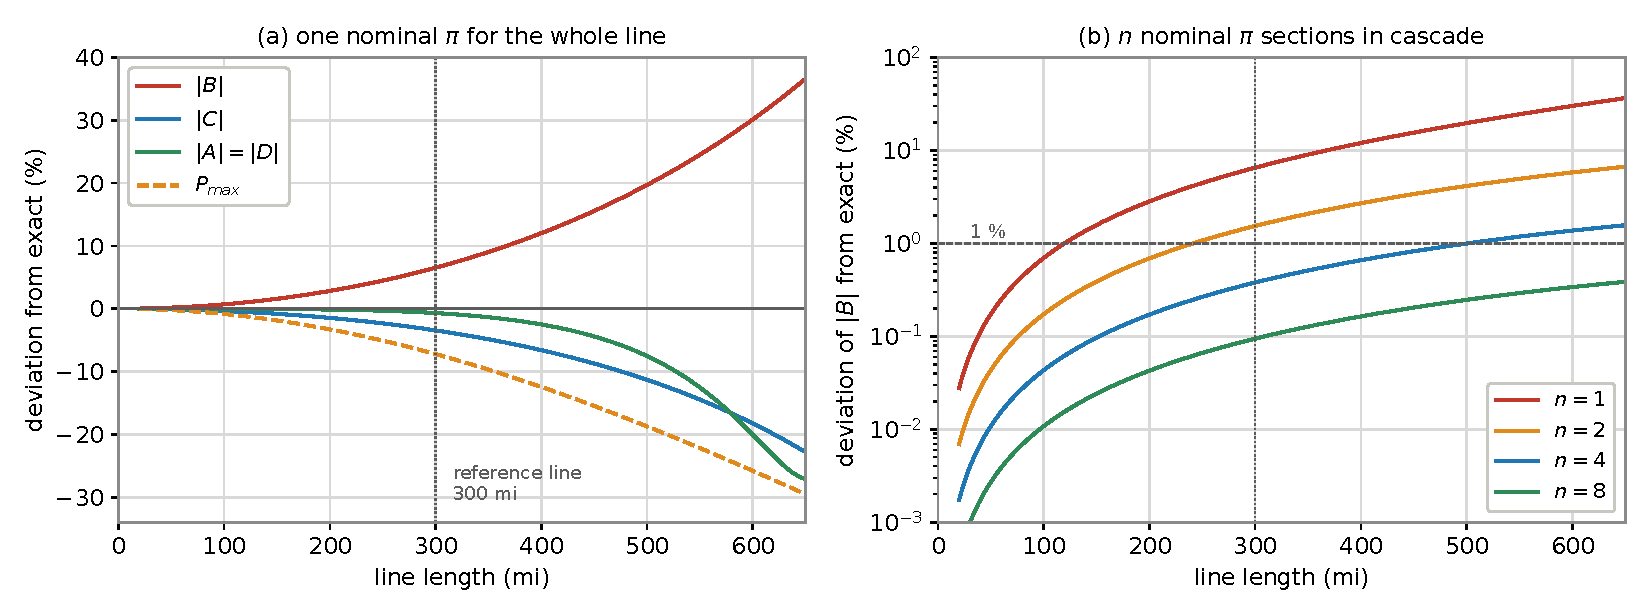
\includegraphics[width=\linewidth]{ac-transmission/fig/tp_model_error.pdf}
  \caption{(a) Deviation of the nominal $\pi$ against line length;
           (b) the same deviation of $\left|\underline{B}\right|$ when the
           line is built from $n$ cascaded $\pi$-sections. Both stop short
           of the quarter wavelength, where $\left|\underline{A}\right|$
           passes through zero}
  \label{fig:ref-model-error}
\end{figure}

\FloatBarrier

\subsubsection{Cascading shorter sections}
\label{sec:ref-cascade}

One lumped section cannot represent a distributed parameter. A second
approach divides the line into $n$ pieces of length $l/n$, models each as
its own nominal $\pi$, and connects the two-ports in cascade. The chain
matrices multiply, so the whole line is
\begin{equation}
  \underline{T} = \left[\underline{T}_{\pi}
    \left(\frac{l}{n}\right)\right]^{n}
  \label{eq:ref-cascade}
\end{equation}
a single matrix power rather than $n$ separate models. Each section covers a
shorter length and therefore deviates less, and as $n \to \infty$ the
product tends to the distributed solution of~\eqref{eq:ac-abcd-exact}.

Table~\ref{tab:ref-cascade} and Figure~\ref{fig:ref-model-error}(b) give
the convergence. Once the sections are electrically short the deviation
falls with $1/n^2$, so doubling $n$ divides it by four. The deviation is set
by the electrical length of a \emph{section} and not by that of the line: on
this conductor, sections of about 120\,mi hold
$\left|\underline{B}\right|$ within 1\,\% at any total length, the same
length that Table~\ref{tab:ref-pi-abs} gives for an undivided line.

\begin{table}[!ht]
  \centering
  \begin{tabular}{@{}r l r r r r r@{}}
    \toprule
    \textbf{$n$} & \textbf{section}
      & \multicolumn{5}{c}{deviation of $\left|\underline{B}\right|$, \%} \\
    \cmidrule(lr){3-7}
    & & \multicolumn{1}{c}{100\,mi} & \multicolumn{1}{c}{200\,mi}
      & \multicolumn{1}{c}{300\,mi} & \multicolumn{1}{c}{400\,mi}
      & \multicolumn{1}{c}{600\,mi} \\
    \midrule
     1 & $l$      & $+0.70$ & $+2.83$ & $+6.53$ & $+12.03$ & $+30.13$ \\
     2 & $l/2$    & $+0.17$ & $+0.69$ & $+1.54$ &  $+2.71$ &  $+5.81$ \\
     4 & $l/4$    & $+0.04$ & $+0.17$ & $+0.38$ &  $+0.66$ &  $+1.38$ \\
     8 & $l/8$    & $+0.01$ & $+0.04$ & $+0.09$ &  $+0.16$ &  $+0.34$ \\
    16 & $l/16$   & $+0.00$ & $+0.01$ & $+0.02$ &  $+0.04$ &  $+0.08$ \\
    \bottomrule
  \end{tabular}
  \caption{Nominal $\pi$-sections in cascade: deviation of
           $\left|\underline{B}\right|$ from the exact two-port against the
           number of sections~[12]}
  \label{tab:ref-cascade}
\end{table}

The equivalent $\pi$ of~\eqref{eq:ac-equivalent-pi} reaches the same result
with one section and no deviation at any length. On this line at 300\,mi it
moves the series branch from $27.5 + j\,162.2\,\Omega$ to $24.1 +
j\,152.5\,\Omega$ and the shunt branch from 1.156 to 1.193\,mS at each end;
at 600\,mi from $54.9 + j\,324.4\,\Omega$ to $30.4 + j\,251.0\,\Omega$ and
from 2.312 to 2.650\,mS. Sixteen cascaded nominal sections still deviate by
0.08\,\% on $\left|\underline{B}\right|$ and require sixteen matrix
products.

Cascading applies where a single equivalent $\pi$ does not.

\begin{itemize}
  \setlength{\itemsep}{0.35em}
  \item \textbf{Something is connected part-way along.} A midpoint series
        bank is a two-port cascaded between two half-lines,
        Section~\ref{sec:series-compensation}, and a tapped substation or a
        transposition point divides the line in the same way. The
        equivalent $\pi$ describes a line between its own two ends and
        nothing else.
  \item \textbf{Quantities along the line are wanted.} The voltage profiles
        of Section~\ref{sec:np-profile} are the intermediate port
        quantities of a cascade; a single two-port gives only its terminals.
  \item \textbf{The line is not uniform.} Different conductor, spacing or
        bundle over part of the route gives each part its own matrix, and
        the product handles it with no extra theory. The equivalent $\pi$
        assumes one $\underline{\gamma}$ and one $\underline{Z}_w$ over the
        whole length.
  \item \textbf{A time-domain or frequency-sweep model is wanted.} The
        cascade is a lumped circuit a simulator can integrate directly,
        which is why electromagnetic-transient models still use chained
        sections rather than a closed-form $\cosh$.
\end{itemize}

Where the line is uniform and only its terminals matter, the equivalent
$\pi$ is the right model, and the cascade is a way of understanding where it
comes from. Appendix~\ref{sec:tp-interconnection} sets the cascade beside
the other ways two-ports combine, which are not interchangeable with it.

\subsubsection{Comparison of the three representations}
\label{sec:ref-models}

Table~\ref{tab:ref-models} evaluates the two-port parameters and the crest
of the power-angle curve for the same line under the three representations
of Section~\ref{sec:ac-transmission}. The simplification
of~\eqref{eq:ac-simple} moves the maximum from $81.0^\circ$ to $90^\circ$
and overstates it by 13\,\%; the nominal $\pi$ keeps the angle but
understates the maximum by 7\,\%, because its $\left|\underline{B}\right|$
is too large. At 300\,mi $\left|\underline{A}\right| = 0.82$, 18\,\% below
the unity that the single series impedance of~\eqref{eq:ac-simple} assumes.
The numbers follow from the model of
Section~\ref{sec:ac-transmission} implemented in~[11].

\begin{table}[!ht]
  \centering
  \begin{tabular}{@{}l r r r r@{}}
    \toprule
    \textbf{Model} & \multicolumn{1}{c}{\textbf{$\left|A\right|$}}
      & \multicolumn{1}{c}{\textbf{$\vartheta_B$}}
      & \multicolumn{1}{c}{\textbf{$\left|B\right|$}}
      & \multicolumn{1}{c}{\textbf{$P_{max}$}} \\
    & & \multicolumn{1}{c}{$^\circ$} & \multicolumn{1}{c}{$\Omega$}
      & \multicolumn{1}{c}{MW} \\
    \midrule
    Short, lossless & 1.000 & 90.0 & 162.2 & 1541 \\
    Nominal $\pi$   & 0.813 & 80.4 & 164.5 & 1266 \\
    Distributed     & 0.819 & 81.0 & 154.4 & 1364 \\
    \bottomrule
  \end{tabular}
  \caption{Two-port parameters and maximum transfer at 300\,mi, both
           terminals at 1.0\,p.u.}
  \label{tab:ref-models}
\end{table}

\subsubsection{The surrounding system}
\label{sec:ref-scr}

The reactance that appears in~\eqref{eq:ac-simple} is the whole path between
the two internal voltages, not the line:
\begin{equation}
  X_{tot} = X_{th\_s} + X_{tr\_s} + X' + X_{tr\_r} + X_{th\_r},
  \qquad
  X_{th} = \frac{U_n^2}{S_{sc}},
  \qquad
  \mathrm{SCR} = \frac{S_{sc}}{P_n}
  \label{eq:ref-xtot}
\end{equation}
with $X_{th}$ the Thevenin reactance of the system behind a terminal, $X_{tr}$
that of the transformer and $S_{sc}$ the short-circuit level there. Taking the
lossless $P_{max} = U_n^2 / X_{tot}$ with equal systems at both ends and the
transformers neglected, Table~\ref{tab:ref-scr} shows how much of the
capability belongs to the terminals rather than to the line.

\begin{table}[!ht]
  \centering
  \begin{tabular}{@{}l r r r@{}}
    \toprule
    \textbf{SCL, each end} & \multicolumn{1}{c}{\textbf{$X_{th}$}}
      & \multicolumn{1}{c}{\textbf{$X_{tot}$}}
      & \multicolumn{1}{c}{\textbf{$P_{max}$}} \\
    \multicolumn{1}{c}{GVA} & \multicolumn{1}{c}{$\Omega$}
      & \multicolumn{1}{c}{$\Omega$} & \multicolumn{1}{c}{MW} \\
    \midrule
    5      & 50.0 & 253.4 &  986 \\
    10     & 25.0 & 203.4 & 1229 \\
    20     & 12.5 & 178.4 & 1401 \\
    stiff  &  0.0 & 153.4 & 1630 \\
    \bottomrule
  \end{tabular}
  \caption{Effect of the surrounding system on the maximum transfer of the
           300\,mi reference line, $X' = 153.4\,\Omega$, transformers
           neglected}
  \label{tab:ref-scr}
\end{table}

A quarter of the capability of this line into 10\,GVA systems is lost to the
terminals rather than to the line itself, which is why a loadability figure
quoted for a line in isolation overstates it. The same quantity, normalised
as the short-circuit ratio, is what governs converter performance on a DC
link.

\subsubsection{Scope of $P_{max}$}
\label{sec:ref-caveat}

$P_{max}$ is not a transfer capability. It is the crest of the power-angle
curve of an uncompensated line between two stiff systems, at an angle
outside the operating range. The transfer the line can carry follows from
the thermal rating of the conductors, the permissible voltage drop and the
angular stability margin, evaluated on the contingency network rather than
the intact one. Section~\ref{sec:limits} covers those limits; the
representation of Section~\ref{sec:ac-transmission} is what they are
evaluated on.

\FloatBarrier

% =============================================================
%  Natural power (surge-impedance loading)
%  Figures in fig/, copied from presentation/design/ac-transmission/fig/
%  (np_*.pdf), generated by that folder's natural_power_figures.py
%  from the exact two-port equations and cross-checked against a
%  20-segment pandapower model (deviation < 0.1 %).
%  Worked line of this section: 400 kV, 2x bundle, 50 Hz, 400 km --
%  not the 500 kV line of Section 6.
% =============================================================
\subsection{Natural Power}
\label{sec:natural-power}

\subsubsection{Definition}
\label{sec:np-definition}

A line terminated in its own wave impedance carries its \emph{natural
power}: the reactive power generated by the shunt capacitance exactly
cancels the reactive power consumed by the series inductance, the line
exchanges no reactive power with either end, and its voltage magnitude stays
constant along the route. North American practice calls the same quantity
the surge-impedance loading, SIL.

On an overhead line $\omega \cdot L' \gg R'$ and $\omega \cdot C' \gg G'$,
so the wave impedance of~\eqref{eq:ac-gamma-zw} is within about a percent of
the real quantity $\sqrt{L'/C'}$, and it is that real value the natural
power is quoted from:
\begin{equation}
  Z_w \approx \sqrt{\frac{L'}{C'}}
  \qquad
  P_{nat} = \mathrm{SIL} = \frac{U^2}{Z_w}
  \label{eq:np-definition}
\end{equation}

$Z_w$ is a property of the conductor geometry alone. It does not depend on
the length of the line, and in the lossless form not on frequency either.
$P_{nat}$ is therefore a reference rather than a rating: below it the line
is a net source of reactive power, above it a net sink.

The same result follows from the two-port equations. Closing the line with
$\underline{Z}_w$ makes $\underline{I}_R = \underline{U}_R /
\underline{Z}_w$, and~\eqref{eq:ac-u-x} and~\eqref{eq:ac-i-x} collapse to a
single travelling wave with no reflection,
\begin{equation}
  \underline{U}(x) = \underline{U}_R \cdot
      e^{\underline{\gamma} \cdot x},
  \qquad
  \underline{I}(x) = \underline{I}_R \cdot
      e^{\underline{\gamma} \cdot x}
  \label{eq:np-matched}
\end{equation}
so that $\underline{U}/\underline{I} = \underline{Z}_w$ everywhere and the
magnitude falls only by the attenuation $e^{-\alpha \cdot l}$,
Figure~\ref{fig:np-matched}. Only the complex $\underline{Z}_w$ matches
perfectly; terminating in the real $\sqrt{L'/C'}$ leaves a small residual
reflection.

\begin{figure}[!ht]
  \centering
  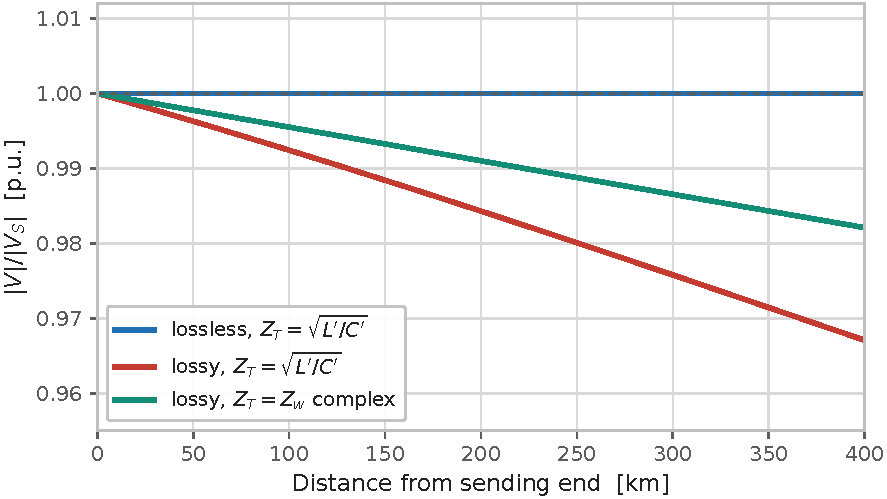
\includegraphics[width=0.78\linewidth]{ac-transmission/fig/np_matched_profile.pdf}
  \caption{Voltage along a line closed in its wave impedance: the profile is
           flat apart from the attenuation, and the residual ripple of the
           real-valued termination}
  \label{fig:np-matched}
\end{figure}

\subsubsection{The reactive balance}
\label{sec:np-balance}

Read as a reactive power balance, a line of length $l$ at line-to-line
voltage $U$ carrying phase current $I$ generates and consumes
\begin{equation}
  Q_C = \omega \cdot C' \cdot l \cdot U^2
  \qquad
  Q_L = 3 \cdot \omega \cdot L' \cdot l \cdot I^2
  \label{eq:np-qcql}
\end{equation}
Natural loading is where the two cancel. Setting $Q_C = Q_L$ eliminates both
$l$ and $\omega$ and gives $I = U / \left(\sqrt{3} \cdot Z_w\right)$, hence
$P_{nat} = \sqrt{3} \cdot U \cdot I = U^2 / Z_w$ again. The cancellation is
independent of length, which is why the natural power is a property of the
cross-section and not of the route.

The worked line of this section is a 400\,kV, 50\,Hz line of 400\,km with a
two-conductor bundle, $R' = 25$\,m$\Omega$/km, $X' = 0.30\,\Omega$/km and
$C' = 12.5$\,nF/km, giving $L' = 0.955$\,mH/km, $Z_w = 276.4\,\Omega$,
$\left|\underline{Z}_w\right| = 276.9\,\Omega$, $\beta \cdot l = 24.88^\circ$
and $P_{nat} = 579$\,MW. It is not the 500\,kV line of
Section~\ref{sec:reference-line}.

Losses move the balance. On the lossless line the zero crossing of the net
reactive flow reproduces $U^2 / Z_w$ to six decimals; on the real line it
falls to 566\,MW, 2.2\,\% below. The sending-end current carries the load
plus the losses, so $3 \cdot I^2 \cdot X' \cdot l$ is larger and the balance
is reached at a lower transfer. Figure~\ref{fig:np-balance} plots the net
reactive flow of both against the transfer.

\begin{figure}[!ht]
  \centering
  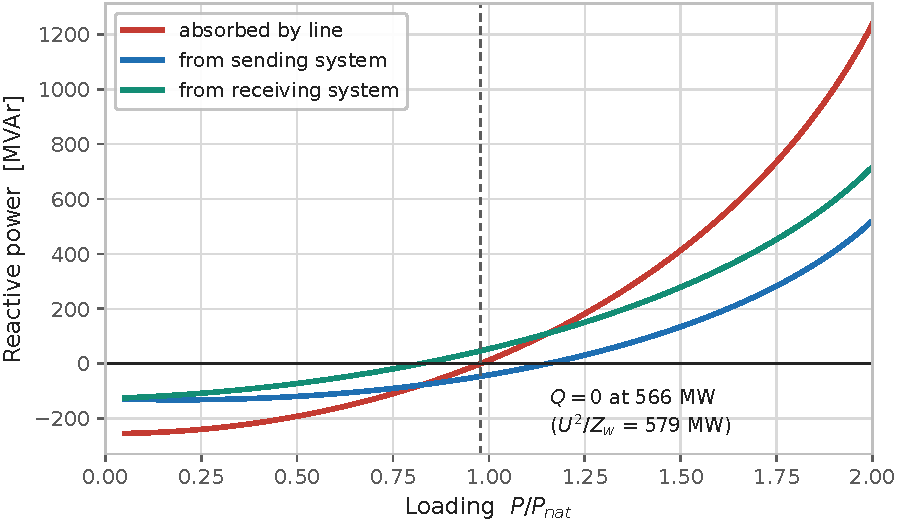
\includegraphics[width=0.78\linewidth]{ac-transmission/fig/np_reactive_balance.pdf}
  \caption{Net reactive power absorbed by the line against transfer,
           $Q_{line} = \Im\left\{\underline{S}_S\right\} -
           \Im\left\{\underline{S}_R\right\}$, lossless and real line}
  \label{fig:np-balance}
\end{figure}

\subsubsection{Voltage profile}
\label{sec:np-profile}

With both terminals held at 1.0\,p.u.\ and the transmission angle solved for
each loading, the profile along the line shows the balance directly,
Figure~\ref{fig:np-profile}. Below $P_{nat}$ the shunt capacitance dominates
and the middle of the line rises, to 1.024\,p.u.\ at no load. At $P_{nat}$
the profile is flat to four decimals. Above it the series reactance
dominates and the middle sags, to 0.873\,p.u.\ at $2 \cdot P_{nat}$, by
which point the angle across the line has reached $63^\circ$.

\begin{figure}[!ht]
  \centering
  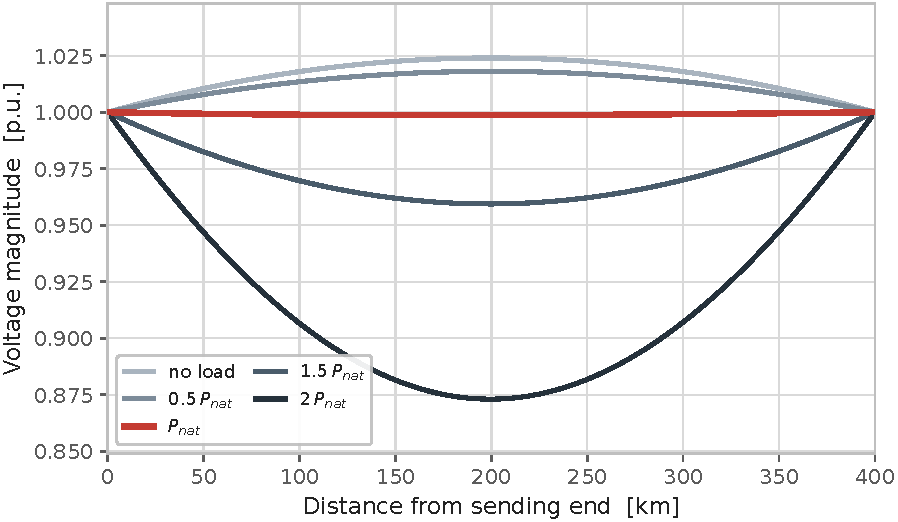
\includegraphics[width=0.78\linewidth]{ac-transmission/fig/np_voltage_profile.pdf}
  \caption{Voltage profile along the 400\,km line at several loadings, both
           terminals at 1.0\,p.u.}
  \label{fig:np-profile}
\end{figure}

\FloatBarrier

\subsubsection{Typical values}
\label{sec:np-typical}

Table~\ref{tab:np-typical} gives the natural power of common line types.

\begin{table}[!ht]
  \centering
  \begin{tabular}{@{}l r r r r r@{}}
    \toprule
    \textbf{Line} & \multicolumn{1}{c}{\textbf{$U$}}
      & \multicolumn{1}{c}{\textbf{$C'$}}
      & \multicolumn{1}{c}{\textbf{$Z_w$}}
      & \multicolumn{1}{c}{\textbf{$P_{nat}$}}
      & \multicolumn{1}{c}{\textbf{$S_{th}/P_{nat}$}} \\
    & \multicolumn{1}{c}{kV} & \multicolumn{1}{c}{nF/km}
      & \multicolumn{1}{c}{$\Omega$} & \multicolumn{1}{c}{MW} & \\
    \midrule
    230\,kV, $1\times$ Drake  & 230 &  9.0 & 376.1 &  141 & 2.8 \\
    345\,kV, $2\times$ bundle & 345 & 11.8 & 292.3 &  407 & 2.6 \\
    400\,kV, $2\times$ bundle & 400 & 12.5 & 276.4 &  579 & 2.4 \\
    500\,kV, $3\times$ bundle & 500 & 13.5 & 256.6 &  974 & 2.3 \\
    765\,kV, $4\times$ bundle & 765 & 13.5 & 250.8 & 2334 & 2.0 \\
    \bottomrule
  \end{tabular}
  \caption{Natural power of typical line types}
  \label{tab:np-typical}
\end{table}

Three things follow. $Z_w$ spans only 251 to 376\,$\Omega$ across the whole
range while $P_{nat}$ spans 141 to 2334\,MW, because $P_{nat}$ is a $U^2$
quantity: voltage, not geometry, sets the transfer. Bundling and tighter
phase spacing are the only levers on $Z_w$, and they work on both terms, 
lowering $L'$ and raising $C'$. And the ratio of thermal rating to natural
power, $S_{th}/P_{nat}$, sets the extent of the thermal plateau of the
loadability curve of Section~\ref{sec:limits}.

AC cables sit at $Z_w \approx 20 \ldots 40\,\Omega$, so their natural power
exceeds the thermal rating and is never reached; as
Section~\ref{sec:cable} sets out, the charging current binds first.

\subsubsection{Light load: the Ferranti effect}
\label{sec:np-ferranti}

On an open-ended line $\underline{I}_R = 0$ and the terminal voltage ratio
follows from~\eqref{eq:ac-abcd-exact} as
\begin{equation}
  \frac{\underline{U}_R}{\underline{U}_S}
    = \frac{1}{\cosh\left(\underline{\gamma} \cdot l\right)}
    \;\longrightarrow\;
    \frac{1}{\cos\left(\beta \cdot l\right)}
  \label{eq:np-ferranti}
\end{equation}
in the lossless limit, so the receiving end rises above the sending end. At
$\beta \cdot l = 24.88^\circ$ the open end reaches 1.102\,p.u., drawing
251\,MVAr of charging power. A 60\,\% shunt reactor brings it back to
0.984\,p.u.; full compensation gives 0.918\,p.u., Figure~\ref{fig:np-ferranti}. The degree of compensation
follows from the light-load voltage, but it also moves the natural power.

\begin{figure}[!ht]
  \centering
  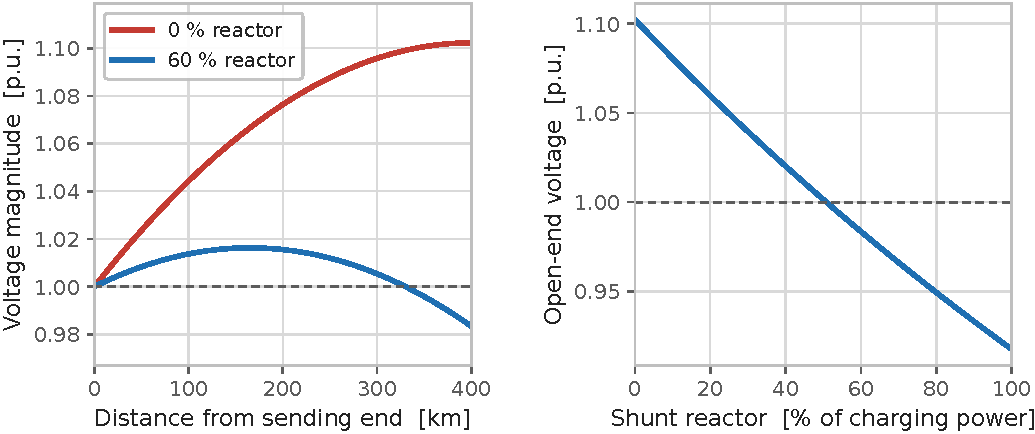
\includegraphics[width=0.74\linewidth]{ac-transmission/fig/np_ferranti.pdf}
  \caption{Open-end voltage rise against line length, and the effect of
           shunt compensation}
  \label{fig:np-ferranti}
\end{figure}

\subsubsection{Effect of compensation on the natural power}
\label{sec:np-compensation}

For uniformly distributed compensation the scaling is exact. Series
compensation of degree $k$ reduces the reactance and shunt compensation of
degree $m$ the capacitance:
\begin{equation}
  X' \to X' \cdot \left(1-k\right)
     \;\Rightarrow\; \frac{P_{nat}}{\sqrt{1-k}},
  \qquad
  C' \to C' \cdot \left(1-m\right)
     \;\Rightarrow\; P_{nat} \cdot \sqrt{1-m}
  \label{eq:np-compensation}
\end{equation}
so $k = 60$\,\% raises $P_{nat}$ by a factor 1.581 and $m = 60$\,\% lowers
it by 0.632, Figure~\ref{fig:np-compensation}.

Real banks are lumped at substations rather than distributed, so these laws
are a first-order guide only. A lumped 30\,\% series bank at $1.4 \cdot
P_{nat}$ on the worked line reduces the transmission angle from $37.6^\circ$
to $25.6^\circ$ and turns the sending-end reactive flow from $+89$ to
$-30$\,MVAr. Section~\ref{sec:series-compensation} treats the lumped case
properly.

\begin{figure}[!ht]
  \centering
  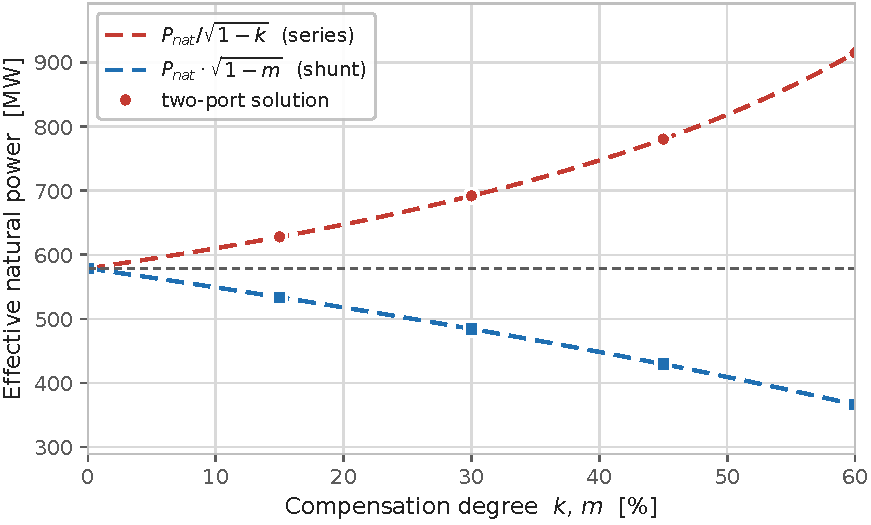
\includegraphics[width=0.74\linewidth]{ac-transmission/fig/np_compensation.pdf}
  \caption{Effect of distributed series and shunt compensation on the
           natural power}
  \label{fig:np-compensation}
\end{figure}

\FloatBarrier

% =============================================================
%  Transmission limits — thermal, voltage drop, angular stability
%  Figures in fig/, copied from presentation/design/ac-transmission/fig/
%  (tl_*.pdf, np_loadability.pdf), generated by that folder's
%  transmission_limits_figures.py and natural_power_figures.py from
%  the exact two-port equations.
% =============================================================
\subsection{Transmission Limits}
\label{sec:limits}

The representation of Section~\ref{sec:ac-transmission} says what a line
does, not what it may be asked to do. Three criteria bound the transfer, and
which of them binds depends almost entirely on length.

\subsubsection{The three criteria}
\label{sec:limits-three}

\paragraph{Thermal.} The conductor temperature sets a current, and with it a
transfer that is independent of length:
\begin{equation}
  P_{th} = \sqrt{3} \cdot U_n \cdot I_{th}
  \label{eq:lim-thermal}
\end{equation}
The limiting mechanism is annealing of the aluminium and, more often, loss
of ground clearance through sag. It is the only one of the three that is a
property of the equipment rather than of the system, and it is weather- and
time-dependent, which is what dynamic line rating exploits.

\paragraph{Voltage drop.} The receiving-end voltage has to stay inside its
band under load. Written on the two-port,
\begin{equation}
  U_S = \left|\underline{A} \cdot \underline{U}_R
             + \underline{B} \cdot \underline{I}_R\right|
      \le 1.0\,\text{p.u.}
  \quad\text{with}\quad
  U_R \ge 0.95\,\text{p.u.}
  \label{eq:lim-voltage}
\end{equation}
Beyond natural loading the line is a net consumer of reactive power, and the
drop grows faster than the transfer. Shunt compensation at the receiving end
raises this limit at the cost of a weaker voltage-stability margin.

\paragraph{Steady-state stability.} The transmission angle must stay far
enough below the crest of the power-angle curve that the system survives the
loss of a parallel element. With a midpoint series bank of degree $k$ the
lossless form is
\begin{equation}
  P_{stab} \approx \frac{U^2}{\left(1-k\right) \cdot X_L}
            \cdot \sin\delta_{max}
  \label{eq:lim-stability}
\end{equation}
and a criterion of $\delta_{max} = 30^\circ$ leaves a factor two on the
lossless maximum. Section~\ref{sec:angular-stability} treats this limit
properly, including why the usable value is well below $P_{max}$.

The loadability of the line is the minimum of the three. Plotted against
length it is the St.~Clair curve.

\subsubsection{Loadability of the reference line}
\label{sec:limits-loadability}

Figure~\ref{fig:tl-loadability} evaluates the three criteria on the 500\,kV
reference line of Section~\ref{sec:reference-line} with the exact two-port
relations, for two boundary conditions. In case~(a) the load sits at the
receiving end with no reactive support, which is the classical St.~Clair
configuration. In case~(b) the line runs between two stiff systems with both
terminals held at 1.0\,p.u., which removes the voltage criterion entirely.
The thermal limit is $I_{th} = 3 \times 1300$\,A at 75\,$^\circ$C, giving
$P_{th} = 3377$\,MW against $P_{nat} = 939$\,MW.

\begin{figure}[!ht]
  \centering
  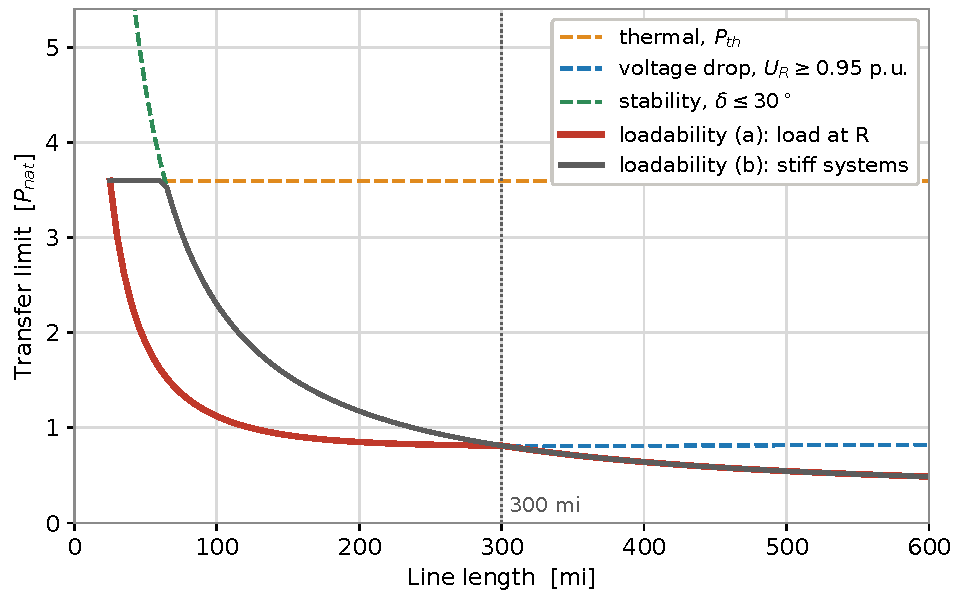
\includegraphics[width=0.78\linewidth]{ac-transmission/fig/tl_loadability.pdf}
  \caption{Loadability of the 500\,kV reference line against length, cases
           (a) and (b), uncompensated}
  \label{fig:tl-loadability}
\end{figure}

In case~(a) the thermal limit binds only to about 25\,mi, after which
voltage drop takes over, and the loadability falls through $1 \cdot P_{nat}$
at 125\,mi. In case~(b) the thermal limit holds to about 60\,mi and angular
stability binds beyond it, with the crossing at 240\,mi. At the 300\,mi
design length both cases give 763\,MW, or $0.81 \cdot P_{nat}$ --- the
voltage and the angle criterion happen to coincide there, and the line
cannot carry even its natural power without compensation.

The boundary condition is not a detail. Holding the receiving end at
1.0\,p.u.\ moves the $1 \cdot P_{nat}$ crossing by 115\,mi on this line. Any
loadability figure has to be quoted with the reactive support it assumes.

\subsubsection{Loadability of the 400\,kV line}
\label{sec:limits-400}

Figure~\ref{fig:np-loadability} repeats the exercise on the 400\,kV, 50\,Hz
line of Section~\ref{sec:natural-power}, with criteria $I \le 2.0$\,kA,
$U_R \ge 0.95$\,p.u.\ and $\vartheta \le 30^\circ$. In case~(a) the thermal
limit holds to 80\,km at $2.3 \ldots 2.4 \cdot P_{nat}$, voltage drop binds
from 120 to 400\,km, angular stability beyond 500\,km, and the curve falls
through $1 \cdot P_{nat}$ at 382\,km. In case~(b) the thermal limit holds to
160\,km, stability binds beyond 200\,km, and the crossing moves to 472\,km.

\begin{figure}[!ht]
  \centering
  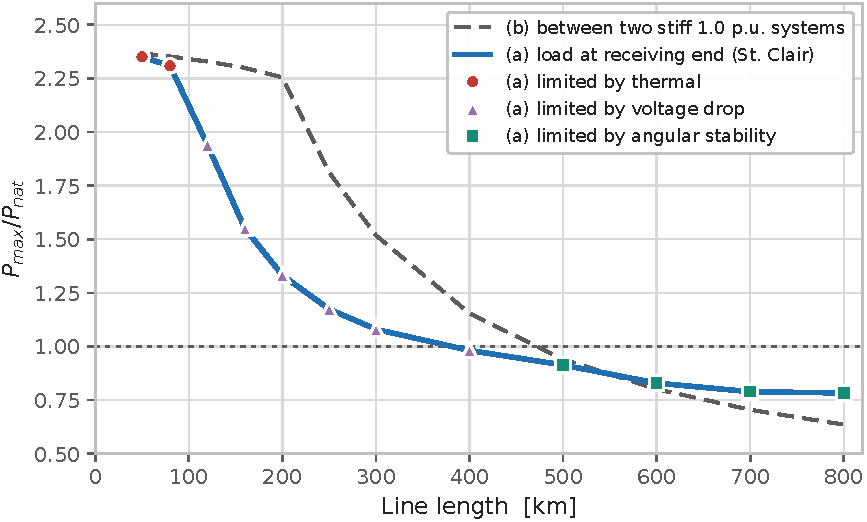
\includegraphics[width=0.78\linewidth]{ac-transmission/fig/np_loadability.pdf}
  \caption{Loadability of the 400\,kV line against length, with $P_{nat}$
           marked}
  \label{fig:np-loadability}
\end{figure}

The shape is the same on both lines: a thermal plateau of about $2 \ldots
2.5 \cdot P_{nat}$ over the first tens of kilometres, then a decay that
crosses natural power somewhere between a quarter and a half of a thousand
kilometres. That is the general statement the St.~Clair curve makes.

\FloatBarrier

\subsubsection{Effect of series compensation}
\label{sec:limits-compensation}

Figure~\ref{fig:tl-loadability-k} repeats case~(b) for a midpoint series
bank of degree $k$, and Table~\ref{tab:tl-k} gives the values at the 300\,mi
design length.

\begin{figure}[!ht]
  \centering
  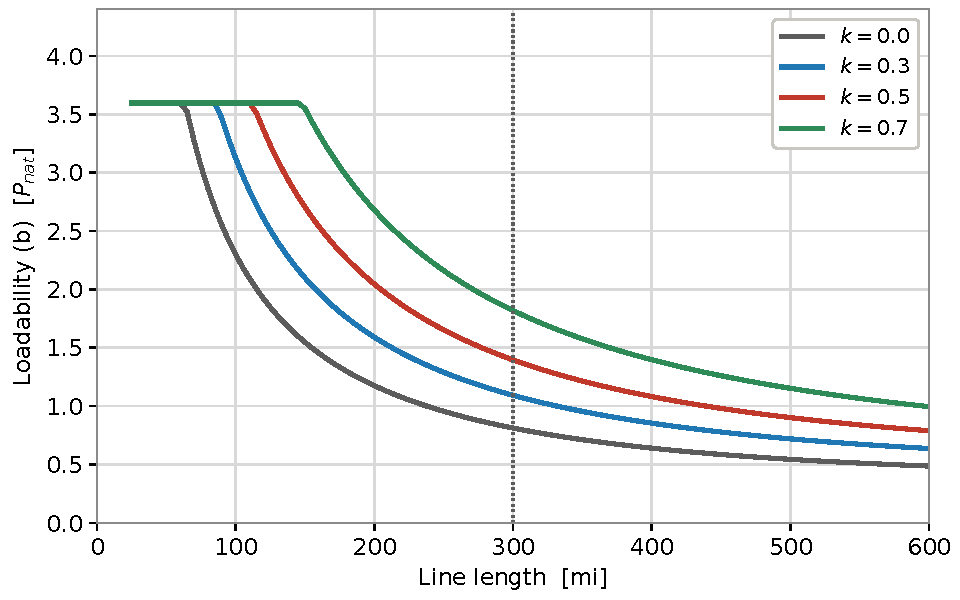
\includegraphics[width=0.74\linewidth]{ac-transmission/fig/tl_loadability_k.pdf}
  \caption{Case (b) loadability of the reference line with a midpoint series
           bank of degree $k$}
  \label{fig:tl-loadability-k}
\end{figure}

\begin{table}[!ht]
  \centering
  \begin{tabular}{@{}c r r r r@{}}
    \toprule
    \textbf{$k$} & \multicolumn{1}{c}{\textbf{$P_{stab}$}}
      & \multicolumn{1}{c}{\textbf{$P_U$}}
      & \multicolumn{1}{c}{\textbf{case (b)}}
      & \multicolumn{1}{c}{\textbf{thermal to}} \\
    & \multicolumn{1}{c}{MW} & \multicolumn{1}{c}{MW}
      & \multicolumn{1}{c}{$P_{nat}$} & \multicolumn{1}{c}{mi} \\
    \midrule
    0   &  763 & 763 & 0.81 &  60 \\
    0.3 & 1027 & 826 & 1.09 &  85 \\
    0.5 & 1311 & 844 & 1.40 & 110 \\
    0.7 & 1708 & 796 & 1.82 & 145 \\
    \bottomrule
  \end{tabular}
  \caption{Effect of a midpoint series bank at 300\,mi on the reference line}
  \label{tab:tl-k}
\end{table}

The bank acts on the stability limit: $k = 0.5$ lifts the 300\,mi
loadability of case~(b) from 0.81 to $1.40 \cdot P_{nat}$. The voltage limit
of case~(a) barely moves, because the $I \cdot X_C$ rise across the bank is
in quadrature with a unity-power-factor load. Series compensation therefore
does not remove the need for reactive support at the receiving end; it
addresses a different limit.

\subsubsection{Equipment limits}
\label{sec:limits-equipment}

The conductor is not always the first thing to run out. Currents follow from
the line-to-line voltage,
\begin{equation}
  I = \frac{S}{\sqrt{3} \cdot U_{LL}}
  \label{eq:lim-current}
\end{equation}
and the switchgear in series with the line carries the same current. The
largest continuous rating available in transmission circuit breakers is
about 5000\,A (Hitachi Energy, GE), so on a high-current scheme the breaker
rating, not the conductor, can set the maximum current and force either a
higher voltage or a second circuit.

\FloatBarrier

% =============================================================
%  Angular stability
%  Figures in fig/, copied from presentation/design/ac-transmission/fig/
%  (as_*.pdf), generated by that folder's angular_stability_figures.py
%  from the exact two-port equations.  Worked line: the 500 kV
%  reference line of Section 6.
% =============================================================
\subsection{Angular Stability}
\label{sec:angular-stability}

Section~\ref{sec:limits} introduced the angular criterion as one of three
bounds. On any line long enough to matter it is the one that binds, and the
margin it needs is larger than the criterion alone suggests.

\subsubsection{Synchronising power}
\label{sec:as-ks}

The meaningful quantity is not the crest of the power-angle curve but its
slope, the \emph{synchronising power coefficient}
\begin{equation}
  K_s = \frac{\partial P}{\partial \delta}
      = \frac{U_S \cdot U_R}{X} \cdot \cos\delta
  \label{eq:as-ks}
\end{equation}
which is the stiffness of the electrical coupling between the machines at
either end. Below the maximum, a rotor that advances delivers more power,
decelerates and returns --- negative feedback. Beyond it, advancing delivers
less power and the machine accelerates further; $K_s = 0$ at the maximum is
therefore the steady-state stability limit in the strict sense.
Figure~\ref{fig:as-power-angle} shows both curves for the reference line.

\begin{figure}[!ht]
  \centering
  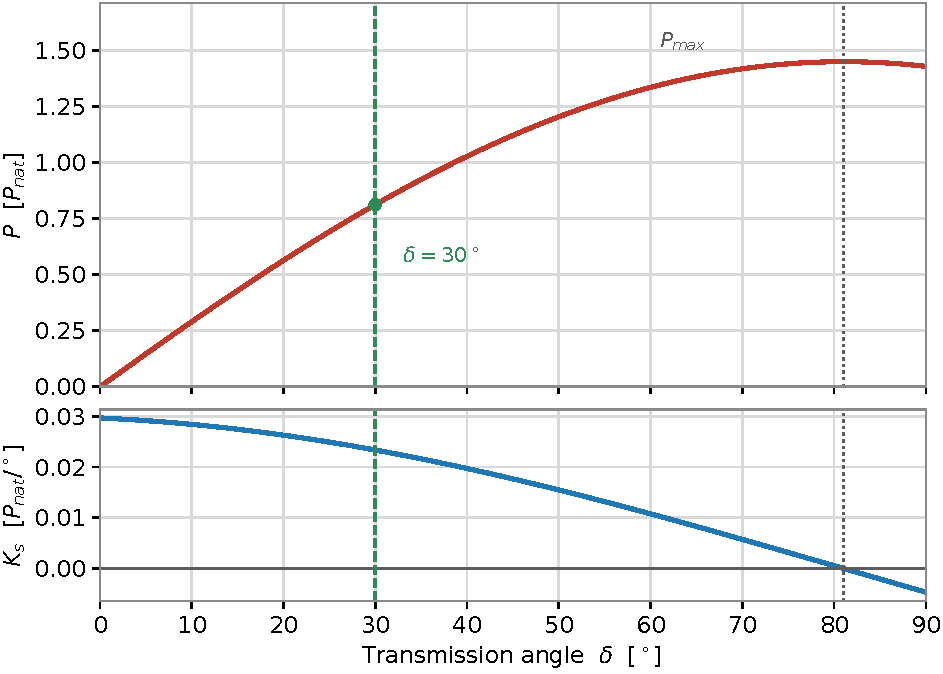
\includegraphics[width=0.74\linewidth]{ac-transmission/fig/as_power_angle.pdf}
  \caption{Power-angle relation and synchronising power coefficient of the
           500\,kV reference line at 300\,mi, both terminals at 1.0\,p.u.}
  \label{fig:as-power-angle}
\end{figure}

With losses the maximum does not fall at $90^\circ$ but at $\delta =
\vartheta_B$, which is $81.0^\circ$ on the reference line. At $\delta =
30^\circ$ the line carries $0.81 \cdot P_{nat}$ with 79\,\% of the stiffness
it has at $\delta = 0$.

Linearising the swing equation about an operating point gives
\begin{equation}
  \frac{2 \cdot H}{\omega_0} \cdot \Delta\ddot{\delta}
  + K_D \cdot \Delta\dot{\delta}
  + K_s \cdot \Delta\delta = 0
  \qquad
  \omega_n = \sqrt{\frac{K_s \cdot \omega_0}{2 \cdot H}}
  \label{eq:as-swing}
\end{equation}
with $H$ the inertia constant and $K_D$ the damping torque coefficient. As
$\delta$ grows, $K_s$ falls, the electromechanical mode slows and its
damping ratio drops. The machine becomes slow and poorly damped before it
loses synchronism, which is why the operating point is held below the
maximum.

\subsubsection{Electrical length}
\label{sec:as-electrical-length}

Above about 250\,km the lumped $\omega \cdot L' \cdot l$
overstates the reactance. The series element of the exact equivalent is
$X' = Z_w \cdot \sin\left(\beta \cdot l\right)$, and substituting into the
lossless maximum gives a clean result:
\begin{equation}
  P_{max} = \frac{U^2}{Z_w \cdot \sin\left(\beta \cdot l\right)}
          = \frac{P_{nat}}{\sin\left(\beta \cdot l\right)}
  \label{eq:as-electrical-length}
\end{equation}
At a quarter wavelength --- 1234\,km on the reference line at 60\,Hz --- the
maximum transfer is exactly $P_{nat}$. That is the analytical spine beneath
the St.~Clair curve, and the reason capability decays with length rather
than staying flat. Figure~\ref{fig:as-electrical-length} compares the three
against length.

\begin{figure}[!ht]
  \centering
  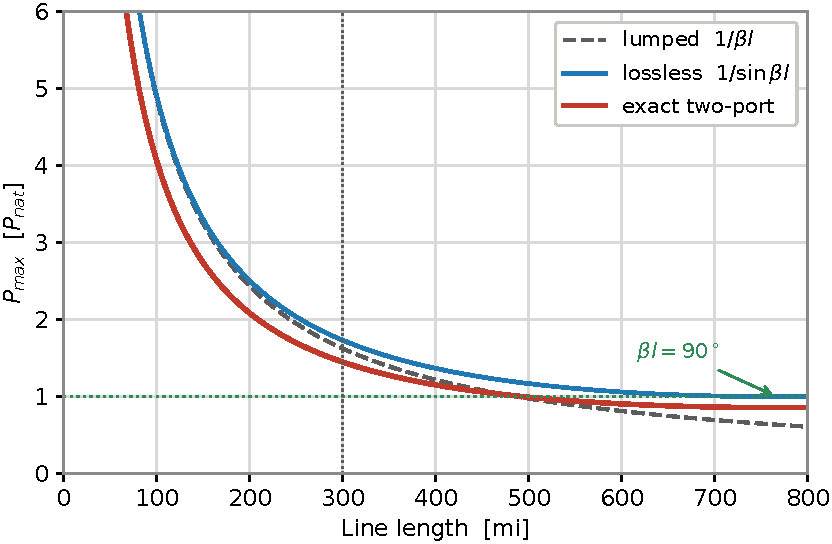
\includegraphics[width=0.74\linewidth]{ac-transmission/fig/as_electrical_length.pdf}
  \caption{Maximum transfer against length: lumped, lossless distributed and
           exact two-port}
  \label{fig:as-electrical-length}
\end{figure}

At the 300\,mi design length $\beta \cdot l = 35.2^\circ$, the lumped
reactance is $162.4\,\Omega$ against $X' = 153.4\,\Omega$, and
$1/\sin\left(\beta \cdot l\right) = 1.73$ against 1.45 for the exact
two-port; losses and charging account for the remaining gap.

\FloatBarrier

\subsubsection{Operating margin below the maximum}
\label{sec:as-contingency}

Two effects cut the usable transfer well below $P_{max}$, and they compound.

The first is the post-contingency network. Two parallel 300\,mi circuits
have $P_{max} = 2726$\,MW intact; losing one doubles the reactance of the
path and leaves 1363\,MW on the survivor. Planning practice requires a
margin of 30 to 35\,\% on the \emph{post-contingency} network,
\begin{equation}
  \frac{P_{max} - P}{P_{max}} \ge 0.30
  \label{eq:as-margin}
\end{equation}
which on this pair allows 954\,MW, or $1.02 \cdot P_{nat}$ for the two
circuits together. A transfer of 1200\,MW looks comfortable intact, at
$\delta = 22.9^\circ$, and sits only 12\,\% below the post-contingency
maximum --- not acceptable. For comparison, the thermal rating of the pair
is 6755\,MW, seven times the binding constraint.
Figure~\ref{fig:as-contingency} shows both power-angle curves.

\begin{figure}[!ht]
  \centering
  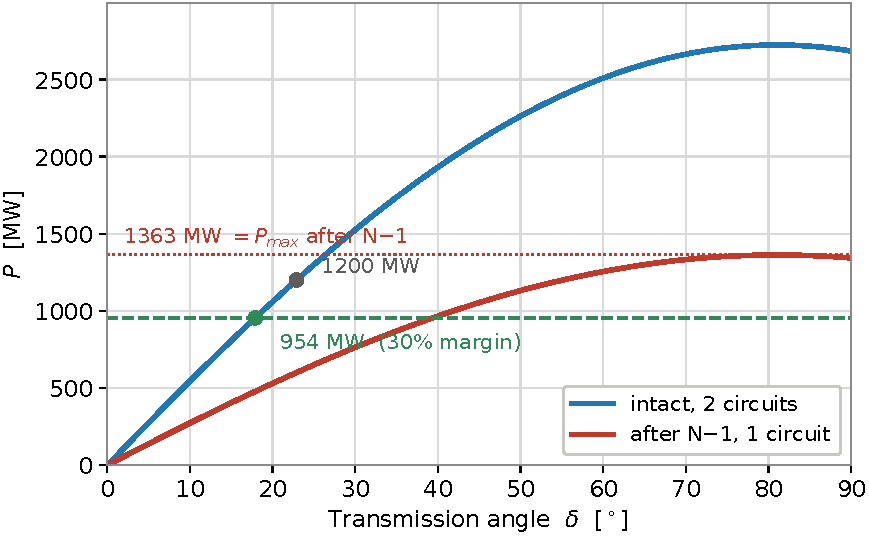
\includegraphics[width=0.74\linewidth]{ac-transmission/fig/as_contingency.pdf}
  \caption{Power-angle curves of two parallel 300\,mi circuits, intact and
           after the loss of one}
  \label{fig:as-contingency}
\end{figure}

\subsubsection{Transient stability}
\label{sec:as-equal-area}

The second effect is the fault case. During a fault the electrical output
collapses while the mechanical input continues; the rotor must give that
energy back before the maximum angle is reached. The equal-area criterion
states the condition as
\begin{equation}
  A_{acc} = \int_{\delta_0}^{\delta_{cc}}
            \left(P_m - P_{flt}\right) \mathrm{d}\delta
  \;=\;
  A_{dec} = \int_{\delta_{cc}}^{\delta_{max}}
            \left(P_{pst} - P_m\right) \mathrm{d}\delta
  \label{eq:as-equal-area}
\end{equation}
with $\delta_{cc}$ the clearing angle. For a machine at $P_m = 0.6$\,p.u.\
with maxima of 1.0 pre-fault, 0.3 during the fault and 0.7 after it,
$\delta_0 = 36.9^\circ$, $\delta_{cc} = 45.5^\circ$ and $\delta_{max} =
121.0^\circ$, Figure~\ref{fig:as-equal-area}.

\begin{figure}[!ht]
  \centering
  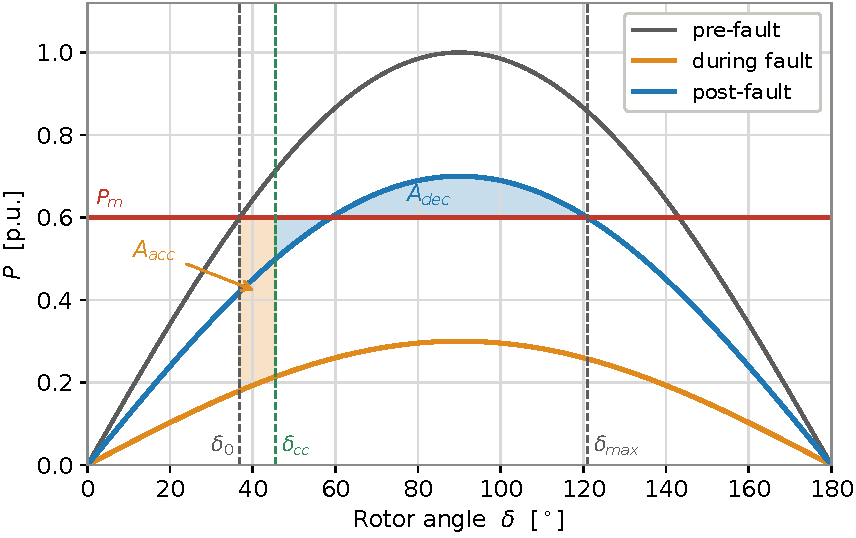
\includegraphics[width=0.72\linewidth]{ac-transmission/fig/as_equal_area.pdf}
  \caption{Equal-area criterion, generic machine per unit}
  \label{fig:as-equal-area}
\end{figure}

A higher pre-fault angle shrinks the decelerating area from both ends at
once, so the critical clearing time falls steeply with loading. This is why
two-cycle breakers and independent-pole tripping buy transfer capability,
and why the transient limit usually binds before the steady-state one.

\FloatBarrier

\subsubsection{Damping}
\label{sec:as-damping}

In a multi-machine system the classical limit generalises to an eigenvalue
criterion. The modes that constrain long transfers are the inter-area modes
at 0.2 to 0.8\,Hz; local plant modes at 0.8 to 2\,Hz and torsional modes at
10 to 45\,Hz. The practical limit is where the damping ratio of a critical
mode falls below about 3 to 5\,\%, which can occur at angles below
$40^\circ$ and therefore below the two-machine maximum.

High-gain automatic voltage regulators, which permit a large angle,
contribute \emph{negative} damping torque at heavy loading. The power system
stabiliser restores it. On a long corridor the available transfer is often
released by tuning the stabiliser rather than by raising $P_{max}$.

\subsubsection{Absence of a transmission angle on a DC link}
\label{sec:as-dc}

A DC link has no transmission angle, no synchronising torque and no
equal-area criterion. The converter control sets power as a commanded
quantity, and length enters only through the conductor resistance, so the
$1/\sin\left(\beta \cdot l\right)$ decay of~\eqref{eq:as-electrical-length}
has no counterpart. An embedded DC link can be modulated to damp the
inter-area modes of the surrounding AC system instead of loading them.

The constraint moves to the terminals: short-circuit ratio and commutation
robustness for line-commutated converters, control interaction for
voltage-sourced ones.

\FloatBarrier

% =============================================================
%  Series compensation
%  Figures in fig/, copied from presentation/design/ac-transmission/fig/
%  (sc_*.pdf), generated by that folder's series_compensation_figures.py
%  from the exact two-port equations with the bank cascaded as a
%  series element.  Worked line: the 500 kV reference line of Section 6.
% =============================================================
\subsection{Series Compensation}
\label{sec:series-compensation}

\subsubsection{Principle}
\label{sec:sc-principle}

A capacitor bank in series with the line cancels part of its inductive
reactance. The degree of compensation is defined against the total series
reactance,
\begin{equation}
  k = \frac{X_C}{X_L},
  \qquad X_L = \omega \cdot L' \cdot l,
  \qquad X_{eff} = \left(1-k\right) \cdot X_L
  \label{eq:sc-k}
\end{equation}
so that the lossless transfer becomes
\begin{equation}
  P = \frac{U^2}{\left(1-k\right) \cdot X_L} \cdot \sin\delta
  \label{eq:sc-power}
\end{equation}
with $\left|U_S\right| = \left|U_R\right| = U$. The line behaves as though
it were shorter: for a given transfer the angle falls and the stability
margin of Section~\ref{sec:angular-stability} rises.

Two properties distinguish it from shunt compensation. The voltage rise
$I \cdot X_C$ across the bank scales with the current, so the compensation
is self-regulating: it appears when it is needed and not at light load. And
it acts on the series branch, which is why it addresses the angular limit
and barely moves the voltage limit of case~(a) in
Section~\ref{sec:limits-compensation}.

The practical range is $k \approx 0.25 \ldots 0.70$. Above that,
sub-synchronous resonance, distance-protection behaviour and bank cost
dominate the choice.

In the two-port model the bank is cascaded as a series element at the point
where it is installed,
\begin{equation}
  \begin{bmatrix} 1 & -j \cdot X_C \\ 0 & 1 \end{bmatrix}
  \label{eq:sc-twoport}
\end{equation}
between the two half-lines for a midpoint bank, which is the arrangement
used throughout this section.

\subsubsection{Single-line arrangement}
\label{sec:sc-sld}

A series bank is not only capacitors. The platform sits at line potential
and carries the full fault current until it is bypassed, so each phase
carries a metal-oxide varistor across the bank to limit the capacitor
voltage under fault current, a bypass breaker with a damping reactor to take
over when the varistor reaches its energy limit, and disconnectors to
isolate the platform. A bypass disconnector keeps the line in service with
the bank out, at $k = 0$. Figure~\ref{fig:sc-sld} shows the arrangement for
one phase, with the bank at the midpoint of the line.

\begin{figure}[!ht]
  \centering
  \begin{tikzpicture}[x=1.07mm, y=1.07mm,
      wire/.style={draw=atFg, line width=0.35mm, line cap=round, line join=round},
      hair/.style={draw=atFg, line width=0.22mm, line cap=round, line join=round},
      bus/.style={draw=atFg, line width=0.9mm, line cap=butt},
      lbl/.style={font=\footnotesize, atFg},
      sub/.style={font=\scriptsize, atFgMuted},
      dot/.style={fill=atFg, circle, inner sep=0pt, minimum size=1.1mm}]
    % buses and line
    \draw[bus] (0,-8) -- (0,8);     \node[lbl,above] at (0,8.5) {S};
    \draw[bus] (120,-8) -- (120,8); \node[lbl,above] at (120,8.5) {R};
    \draw[wire] (0,0) -- (30,0);
    \draw[wire] (90,0) -- (120,0);
    \node[sub] at (15,3.2) {$l/2$};
    \node[sub] at (105,3.2) {$l/2$};
    % line disconnectors into the platform
    \draw[wire] (30,0) -- (33,0);
    \draw[wire] (33,0) -- (38.5,3.5);
    \draw[wire] (39,0) -- (42,0);
    \node[sub,above] at (36,4) {DS1};
    \draw[wire] (78,0) -- (81,0);
    \draw[wire] (81,0) -- (86.5,3.5);
    \draw[wire] (87,0) -- (90,0);
    \node[sub,above] at (84,4) {DS2};
    % main branch: series capacitor
    \node[dot] at (42,0) {};  \node[dot] at (78,0) {};
    \draw[wire] (42,0) -- (57,0);
    \draw[wire] (57,-4) -- (57,4);  \draw[wire] (60,-4) -- (60,4);
    \draw[wire] (60,0) -- (78,0);
    \node[lbl,above] at (58.5,4.8) {$C$\quad{\scriptsize\color{atFgMuted}$X_C = k \cdot X_L$}};
    % MOV branch
    \draw[wire] (42,0) -- (42,-10) -- (54,-10);
    \draw[wire] (54,-13) rectangle (66,-7);
    \draw[hair] (55,-12) -- (65,-8);
    \draw[wire] (66,-10) -- (78,-10) -- (78,0);
    \node[sub,below] at (60,-13.3) {MOV};
    % damping reactor and bypass breaker
    \draw[wire] (42,-10) -- (42,-20) -- (50,-20);
    \draw[wire] (50,-22) rectangle (58,-18);
    \draw[wire] (58,-20) -- (63,-20);
    \draw[wire] (63,-22) -- (67,-18);  \draw[wire] (63,-18) -- (67,-22);
    \draw[wire] (67,-20) -- (78,-20) -- (78,-10);
    \node[sub,below] at (54,-22.3) {$L_d$};
    \node[sub,below] at (65,-22.3) {bypass CB};
    % bypass disconnector around the whole bank
    \draw[wire] (33,0) -- (33,-33) -- (55,-33);
    \draw[wire] (55,-33) -- (60.5,-29.5);
    \draw[wire] (61,-33) -- (87,-33) -- (87,0);
    \node[sub,below] at (58,-34) {bypass DS};
    % platform outline
    \draw[atFgMuted, line width=0.4pt, densely dashed] (39,-27.5) rectangle (81,12.5);
    \node[sub,anchor=south east] at (81,12.8) {capacitor platform, line potential};
    % current arrow
    \draw[-{Stealth[length=2mm]}, atFgMuted] (8,-3.5) -- (22,-3.5)
      node[midway,below,sub] {$I$};
  \end{tikzpicture}
  \caption{Single-line diagram of a midpoint series bank, one phase.
           Symbols to IEC 60617~[18]}
  \label{fig:sc-sld}
\end{figure}

The varistor limits the capacitor voltage under fault current and the bypass
breaker with its damping reactor $L_d$ takes over at the varistor energy
limit. DS1 and DS2 isolate the platform; the bypass disconnector keeps the
line in service with the bank out.

\subsubsection{Effect on the power-angle curve}
\label{sec:sc-power-angle}

Figure~\ref{fig:sc-power-angle} shows the power-angle curves of the 500\,kV
reference line for a midpoint bank at several degrees of compensation, and
Table~\ref{tab:sc-power-angle} the resulting maxima.

\begin{figure}[!ht]
  \centering
  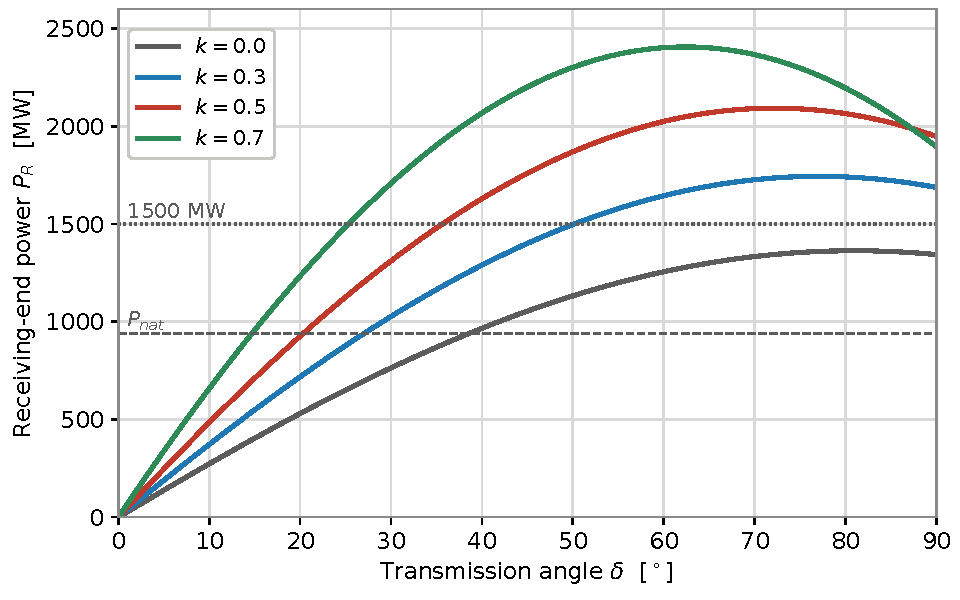
\includegraphics[width=0.74\linewidth]{ac-transmission/fig/sc_power_angle.pdf}
  \caption{Power-angle curves of the reference line with a midpoint series
           bank, both terminals at 1.0\,p.u.}
  \label{fig:sc-power-angle}
\end{figure}

\begin{table}[!ht]
  \centering
  \begin{tabular}{@{}c r r r@{}}
    \toprule
    \textbf{$k$} & \multicolumn{1}{c}{\textbf{$X_C$}}
      & \multicolumn{1}{c}{\textbf{$P_{max}$}}
      & \multicolumn{1}{c}{\textbf{$\delta$ at 1500\,MW}} \\
    & \multicolumn{1}{c}{$\Omega$} & \multicolumn{1}{c}{MW}
      & \multicolumn{1}{c}{$^\circ$} \\
    \midrule
    0   & 0     & 1363 & --- \\
    0.3 & 48.7  & 1744 & 50.1 \\
    0.5 & 81.2  & 2093 & 35.7 \\
    0.7 & 113.7 & 2407 & 25.3 \\
    \bottomrule
  \end{tabular}
  \caption{Midpoint bank on the 300\,mi reference line, exact two-port}
  \label{tab:sc-power-angle}
\end{table}

Uncompensated, 1500\,MW --- $1.6 \cdot P_{nat}$ --- cannot be carried at
all; at $k = 0.5$ it is carried at $36^\circ$. The maximum also moves to
smaller angles as $k$ grows, which is the electrical shortening of the line
expressed on the curve. The lossless form
$U^2 / \left(\left(1-k\right) \cdot X_L\right)$ would give 1540\,MW
uncompensated and 3080\,MW at $k = 0.5$; at this length $R = 27.5\,\Omega$
and the line charging are not negligible, which is why the exact two-port is
used.

\subsubsection{Voltage profile at heavy load}
\label{sec:sc-voltage}

Delivering 900\,MW at $\cos\varphi = 0.95$ lagging with the receiving end
held at 1.0\,p.u., the uncompensated line requires a sending-end voltage of
1.217\,p.u., outside the usual 0.95 to 1.05\,p.u.\ operating band. The
midpoint bank raises the
voltage by $I \cdot X_C$ in the direction of power flow, and the sending end
falls to 1.157, 1.127 and 1.107\,p.u.\ for $k = 0.3$, 0.5 and 0.7,
Figure~\ref{fig:sc-voltage}.

\begin{figure}[!ht]
  \centering
  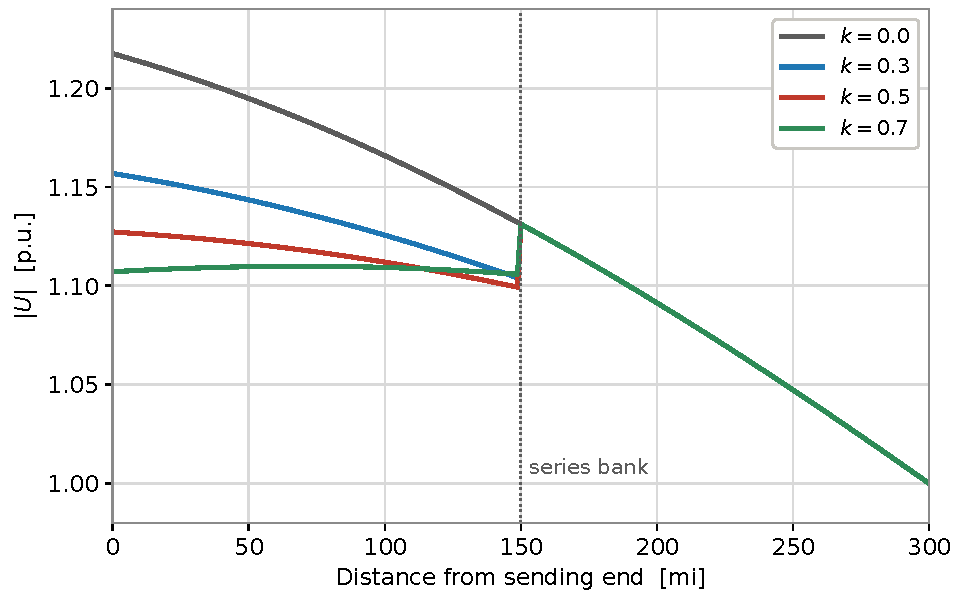
\includegraphics[width=0.74\linewidth]{ac-transmission/fig/sc_voltage_profile.pdf}
  \caption{Voltage profile at heavy load with a midpoint series bank}
  \label{fig:sc-voltage}
\end{figure}

The receiving half of the line is unchanged, because the bank acts only on
what is upstream of it. That is why end-of-line banks and split banks are
also used where the voltage profile rather than the angle is the problem.

\FloatBarrier

\subsubsection{Bank rating and protection}
\label{sec:sc-rating}

The bank is rated for the planned continuous line current, not for the
conductor thermal limit:
\begin{equation}
  U_C = I_{rated} \cdot X_C
  \qquad
  Q_C = 3 \cdot I_{rated}^{2} \cdot X_C
  \label{eq:sc-rating}
\end{equation}
Table~\ref{tab:sc-rating} gives the resulting bank for the reference line at
$k = 0.5$.

\begin{table}[!ht]
  \centering
  \begin{tabular}{@{}l l r@{}}
    \toprule
    \textbf{Quantity} & & \multicolumn{1}{c}{\textbf{Value}} \\
    \midrule
    $k$ & & 0.5 \\
    $X_C$ & $\Omega$ & 81.2 \\
    $C$ per phase & \textmu F & 32.7 \\
    $I_{rated}$ & A & 2000 \\
    \midrule
    $U_C$ per phase & kV & 162 \\
    $Q_C$ three-phase & MVAr & 974 \\
    MOV level ($2.3 \cdot U_C$) & kV & 373 \\
    \bottomrule
  \end{tabular}
  \caption{Midpoint bank rating on the reference line at $k = 0.5$}
  \label{tab:sc-rating}
\end{table}

$I_{rated}$ is taken as about $1.15 \cdot$ the current at 1500\,MW and
500\,kV. The fault-current voltage is limited by the metal-oxide varistor at
a protective level of $2.0 \ldots 2.5 \cdot U_C$, with the bypass breaker
and damping circuit behind it. Emergency ratings --- typically 30\,min and
10\,s --- are specified separately from the continuous rating.

\subsubsection{Sub-synchronous resonance}
\label{sec:sc-ssr}

The bank forms a series resonance with the line and source reactances at
\begin{equation}
  f_{er} = f_0 \cdot \sqrt{\frac{X_C}{X_L + X_S}}
  \label{eq:sc-ssr}
\end{equation}
Rotor currents see the complement $f_0 - f_{er}$, which has to stay clear of
the torsional modes of the turbine-generator shaft --- 10 to 45\,Hz for
large steam units. Figure~\ref{fig:sc-ssr} screens the reference line against
the degree of compensation.

\begin{figure}[!ht]
  \centering
  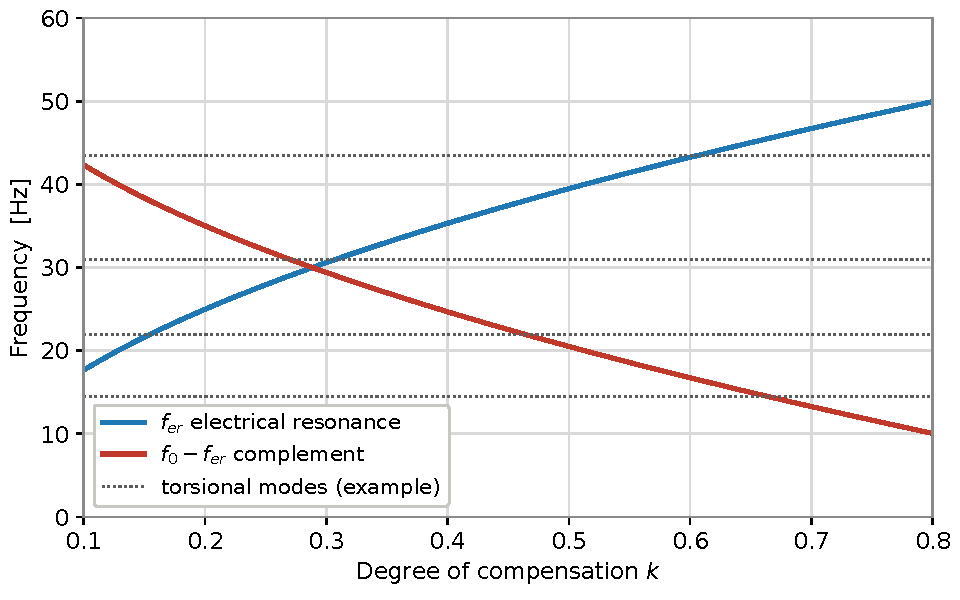
\includegraphics[width=0.72\linewidth]{ac-transmission/fig/sc_ssr_screening.pdf}
  \caption{Sub-synchronous resonance screening: electrical resonance and its
           complement against the degree of compensation}
  \label{fig:sc-ssr}
\end{figure}

With $X_S = 25\,\Omega$, which is 15\,\% on 1500\,MVA, a compensation of
$k = 0.5$ gives $f_{er} = 39.5$\,Hz and a complement of 20.5\,Hz --- within
2\,Hz of an illustrative 22\,Hz torsional mode. A hit at screening level
calls for a detailed study or a different $k$; type-3 wind generation adds
sub-synchronous control interaction to the same screening. The torsional
modes used at this stage are illustrative, and real values come from the
generator manufacturer.

\FloatBarrier

